\documentclass{beamer}
\usepackage[utf8]{inputenc}
\usepackage{hyperref}
\usepackage[T1]{fontenc}
\usepackage{tikz}
\usetikzlibrary{positioning}
\usepackage{transparent}
\usepackage{verbatim}
\newcommand{\semitransp}[2][40]{\textcolor{fg!#1}{#2}}
\usepackage[super]{nth}
\usepackage{listings}
\usepackage{booktabs}
\usepackage{pgf}
\usepackage{lmodern}

\usepackage[absolute,overlay]{textpos}
\usepackage{xcolor}
\usepackage{latexsym,xcolor,multicol,booktabs,calligra}
\usepackage{amsmath,amssymb,BOONDOX-cal,bm}	
\usepackage{pstricks}
\usepackage{stackengine}   
\usepackage{graphicx}
\graphicspath{{figures/}}
\usepackage{romannum}
\usepackage{minted}

\author{\textbf{Antonio Pucciarelli}}
\title{\textsc{Turbomachinery: Compressor preliminary design}}
\institute{Politecnico di Milano} 
\date{\today}
\logo{
\includegraphics[width=0.2\textwidth]{polimiLogo.jpeg}}
\newcommand{\nologo}{\setbeamertemplate{logo}{}}

\usepackage{Wue}

\def\cmd#1{\texttt{\color{red}\footnotesize $\backslash$#1}}
\def\env#1{\texttt{\color{blue}\footnotesize #1}}

\newtheorem{thm}{Theorem}[theorem]

\definecolor{mygreen}{rgb}{0,0.6,0}
\definecolor{mygray}{rgb}{0.5,0.5,0.5}
\definecolor{mymauve}{rgb}{0.58,0,0.82}

\definecolor{codegreen}{rgb}{0,0.6,0}
\definecolor{codegray}{rgb}{0.5,0.5,0.5}
\definecolor{codepurple}{rgb}{0.58,0,0.82}
\definecolor{backcolour}{rgb}{0.95,0.95,0.92}
\definecolor{LightGray}{gray}{0.9}

\begin{document}
	\begin{frame}
    		\titlepage
    	\end{frame}

	\section{Problem Description}
        \begin{frame}{Initial Conditions \& Constraints}
	\begin{block}{Inlet conditions}
		\begin{itemize}
			\item $P_{T0} = 1 bar$
			\item $T_{T0} = 300 K$
		\end{itemize}
	\end{block}
	\begin{alertblock}{Constraints}
		\begin{itemize}
			\item $r_{max} = 0.45 m$
			\item $\beta_{TT} = 1.45$
			\item $\dot{Q} = 100 \frac{kg}{s}$
			\item \textbf{max} $\eta$
		\end{itemize}
	\end{alertblock}
	Due to the \textbf{course track} and \textbf{preference}, the turbomachinery design will be on an \textbf{axial} compressor.
\end{frame}

        
	\section{Similitude}
        \subsection{Procedural Steps}
	\begin{frame}{Procedural Steps}
	\begin{alertblock}{Hypothesis}
		It has been chosen to not use an \textbf{inlet guide vane} for simplicity of design and so $V_{t0} = 0 \frac{m}{s}$ and $\chi$ dictate the behaviour of $\lambda$. Another initial desing choice is to keep, in the similarity/adimensional analysis of the compressor, $V_a$ \textbf{constant} and to \textbf{avoid} using a \textbf{flaring based} approach.
	\end{alertblock}
	\textbf{Main procedural steps:}
	\begin{itemize}
		\item $\lambda$ and $\psi$ computation from $\chi$ and $V_{t0}$
		\item $\phi$ and $\eta$ computation 
		\item $V_a$ and $L_{eu}$ computation from $\phi$, $\beta_{TT}$ and $\eta$
		\item computing \textbf{mean} velocity triangles, using the above hypothesis
		\item computing \textbf{blade height}
	\end{itemize}
	\end{frame}
\subsection{Main Design Quantities}
	\begin{frame}{Graph Analysis: $\chi$ \& $M$}
		\begin{figure}
			\centering
			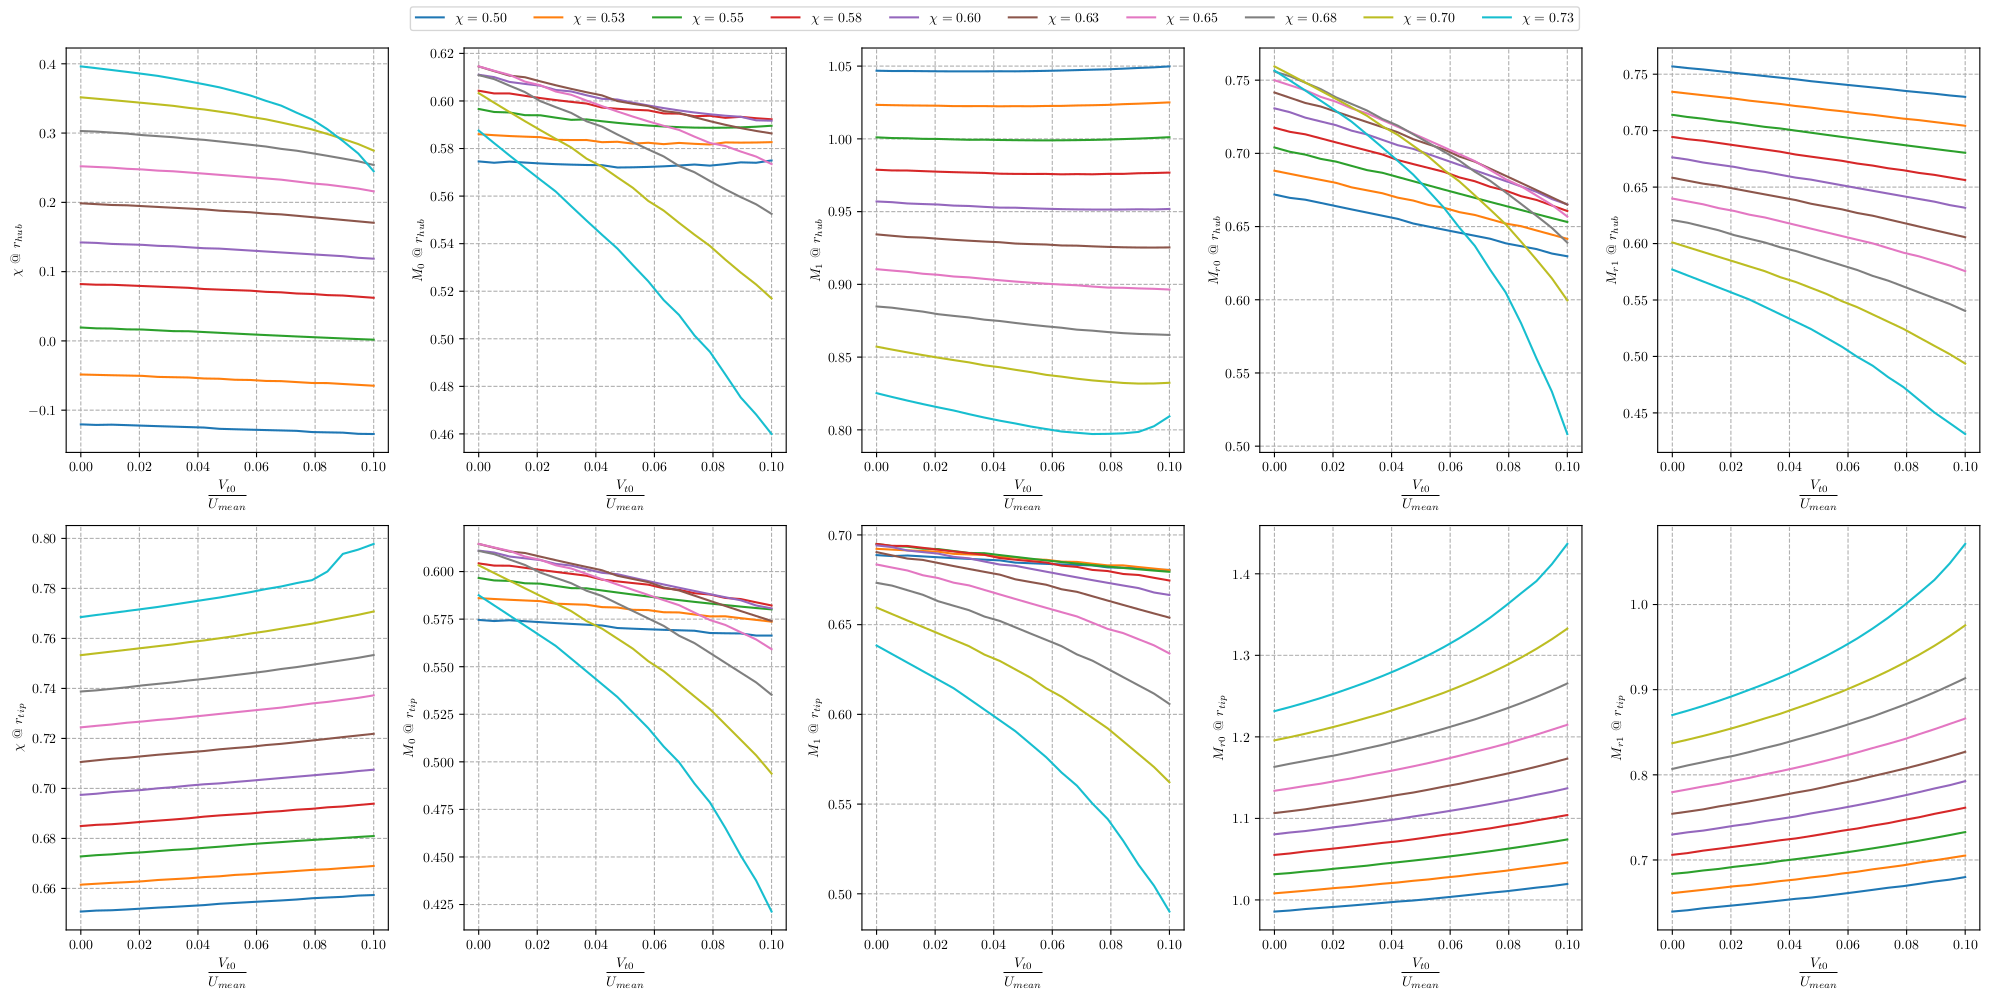
\includegraphics[width=\textwidth]{figures/reactionStudy0.png}
		\end{figure}
	\end{frame}
	\begin{frame}{Graph Analysis: $\alpha$ \& $\beta$}
		\begin{figure}
			\centering
			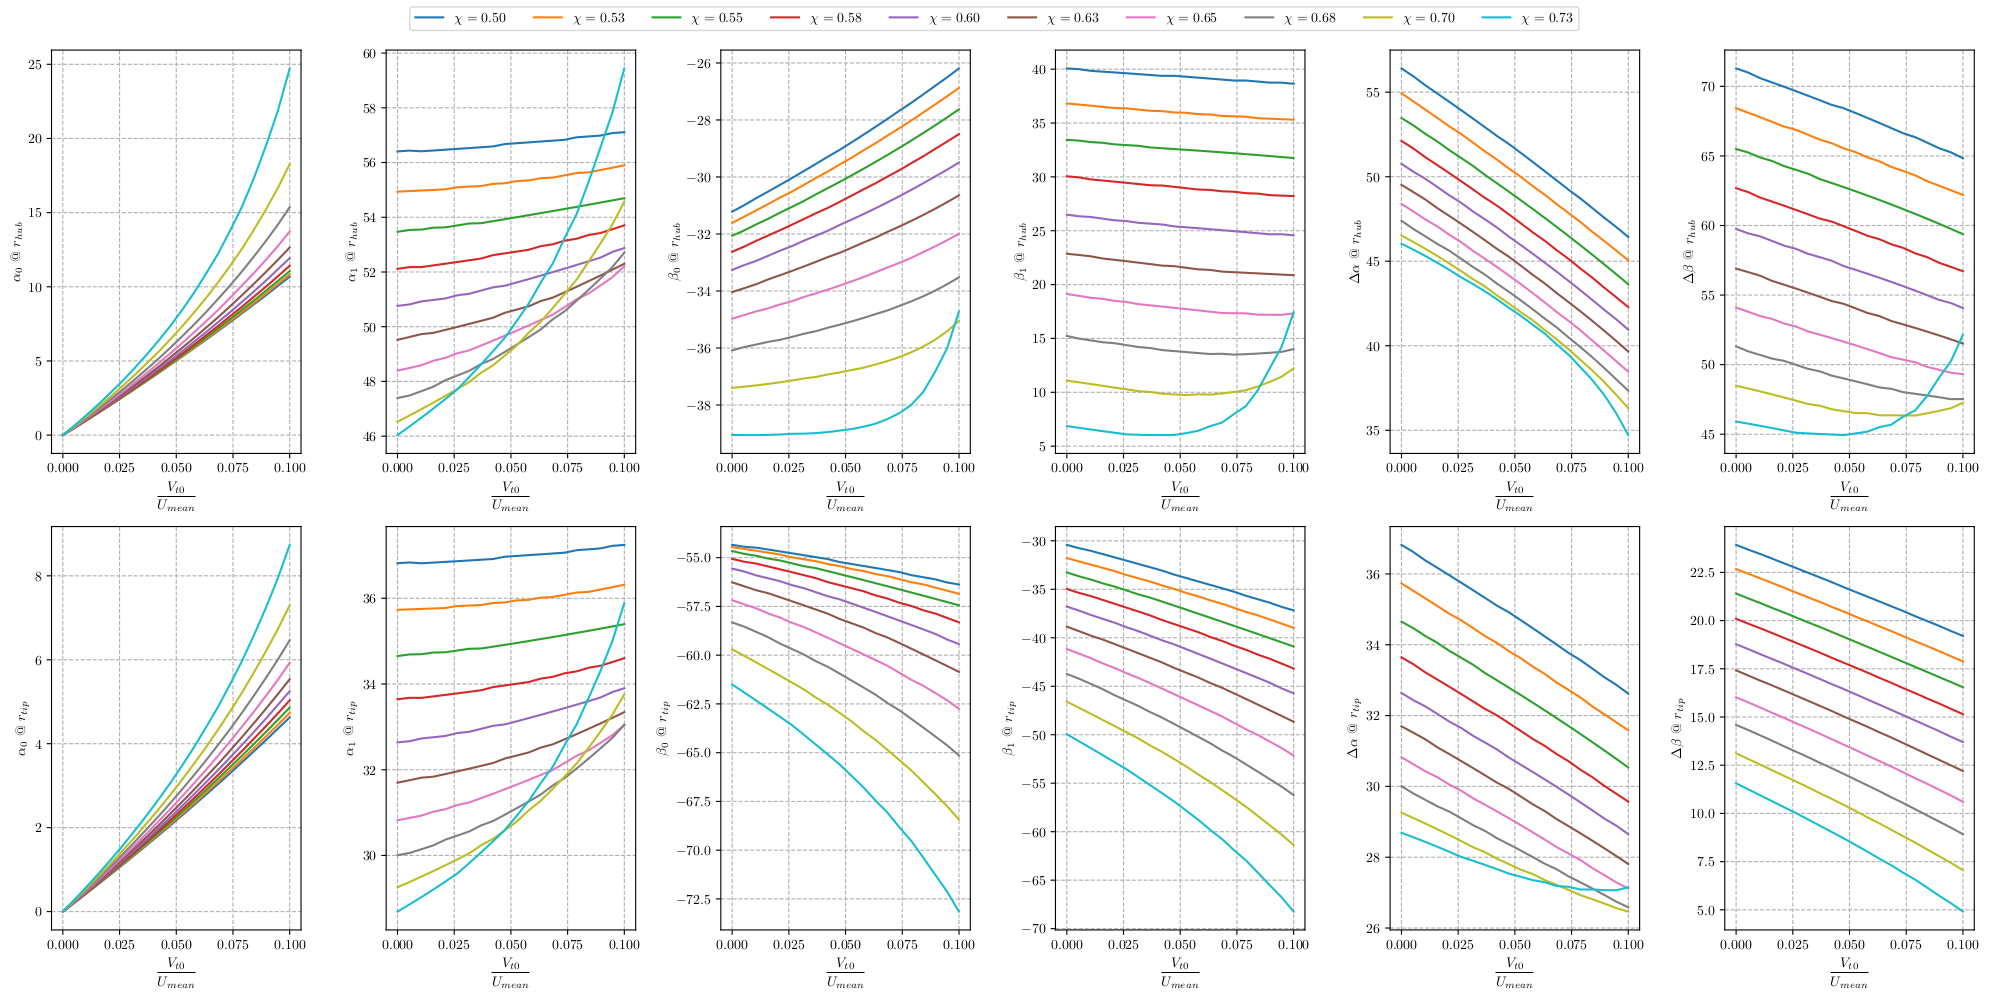
\includegraphics[width=\textwidth]{figures/reactionStudy1.png}
		\end{figure}
	\end{frame}
	\begin{frame}{$\lambda$ \& $\psi$}
		From the previous graphs:
			\begin{itemize}
				\item $\chi = 0.55$
				\item $r_{mean} = 0.325 m$
				\item $\frac{V_t}{U_{mean}} = 0$
			\end{itemize}
		Taking into account the previous modeling hypothesis:
		\begin{align}
			\lambda & = (1 - \chi - \frac{V_t}{U_{mean}}) \cdot 4 \\ 
			\psi    & = \frac{\lambda}{2} 
		\end{align}
	\end{frame}
	
	\begin{frame}{$\phi_{(\psi)}$}
		From \cite[Sec. 10.4]{axial2004} it is imposed that $\frac{W_2}{W_1} \geq 0.7$ with a \textit{safety} margin of $2 \%$.  
		\begin{figure}
			\centering
			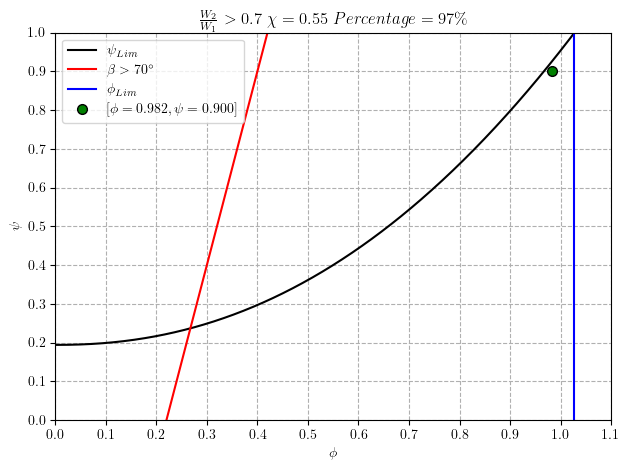
\includegraphics[width=0.7\textwidth]{figures/stagePerf.png}
		\end{figure}
	\end{frame}
	\begin{frame}{$\eta$ \& $L_{eu}$}
		$\eta$ is computed from an \textbf{Lieblein} efficiency chart\footnote{This chart has been interpolated from the course slides charts.} given $\phi$ and $\chi$. This parameter will be used for the computation of $L_{eu}$ given the $\beta_{TT}$ target.
		\begin{columns}
			\column{0.5\textwidth}
				\begin{figure}
					\centering 
					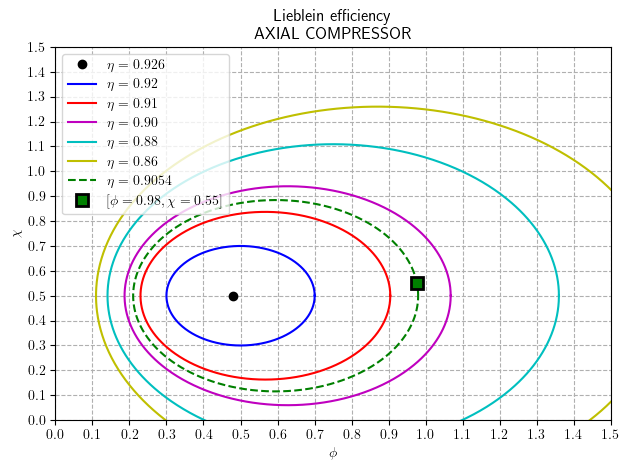
\includegraphics[width=1\textwidth]{figures/efficiency.png}
				\end{figure}
			\column{0.5\textwidth}
			\begin{align}
				L_{is} & = \frac{\gamma \ R}{\gamma - 1} \ T_{in} \ (\beta_{TT}^{{\frac{\gamma - 1}{\gamma}}} - 1) \\
				L_{eu} & = \frac{L_{is}}{\eta}
			\end{align}
		\end{columns}
	\end{frame}
\subsection{$V_{t_{mean}}$, $V_{a_{mean}}$, $U_{mean}$ \& velocity triangles}
\begin{frame}[fragile]
	\begin{align}
		U_{mean} & = \frac{L_{eu}}{\psi} \\ 
		V_{a_{mean}} & = \phi \ U_{mean} \\ 
		L_{eu} & = U_1 \ V_{t1} - U_0 \ V_{t0} \\ 
		       & = U_{1_{mean}} \ V_{t1_{mean}} - U_{0_{mean}} \ V_{t0_{mean}} = U_{mean} \ \Delta V_{t_{mean}} 
	\end{align}
	$\Delta V_t$ computation allows to get a \textit{first sketch} of the \textbf{velocity triangles}.
	The first analysis results are stored in \verb|compressor_0.55_0.325_28_28.txt|.
\end{frame}

{\nologo
\begin{frame}
	\begin{columns}
		\column{0.5\textwidth}
			\begin{figure}
				\centering
				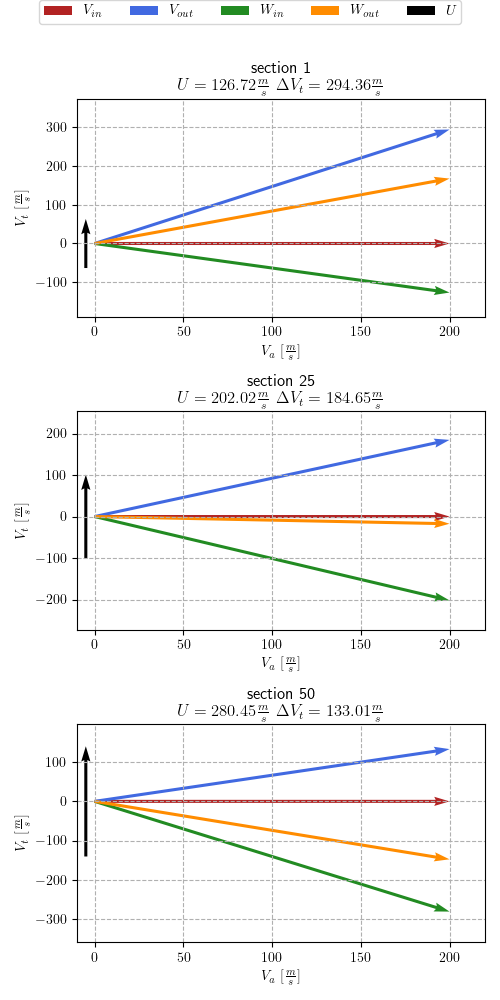
\includegraphics[width=0.7\textwidth]{figures/rotorVelocityTriangle.png}
			\end{figure}
		\column{0.5\textwidth}
			\begin{figure}
				\centering
				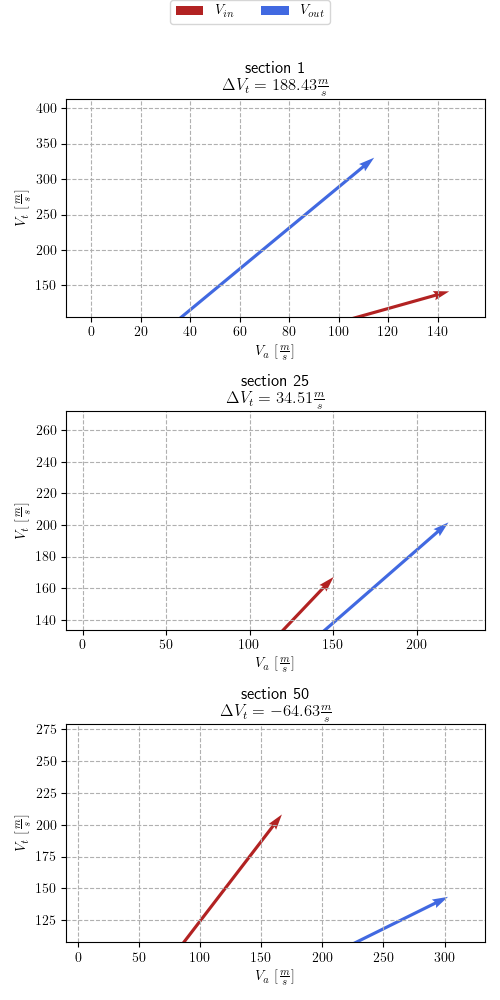
\includegraphics[width=0.7\textwidth]{figures/statorVelocityTriangle.png}
			\end{figure}
	\end{columns}
\end{frame}
}


    
   	\section{Blade Modeling}
        \subsection{Losses Modeling}
\subsubsection{Profile Losses}
	\begin{frame}{Profile Losses}
		The profile losses used are related to the \textbf{Leiblein modeling} approach, \cite[Ch. 6]{axial2004}.
				
	\end{frame}
\subsubsection{Compressibility Losses}
\subsubsection{Shock Losses}
\subsubsection{Tip Leackage Losses}
\subsection{Radial Equilibrium}
\subsubsection{General Formulation}
\subsubsection{Vortex Model}
\subsubsection{$\mathtt{NISRE}$ Equilibrium Results}
\subsection{$\mathtt{turboLIB}$}
\subsubsection{Section Analysis \& Optimization}
\subsubsection{$\mathtt{.stl}$ \& $\mathtt{.scad}$ Generation}



	\section{Efficiency}
	%% Creator: Matplotlib, PGF backend
%%
%% To include the figure in your LaTeX document, write
%%   \input{<filename>.pgf}
%%
%% Make sure the required packages are loaded in your preamble
%%   \usepackage{pgf}
%%
%% Also ensure that all the required font packages are loaded; for instance,
%% the lmodern package is sometimes necessary when using math font.
%%   \usepackage{lmodern}
%%
%% Figures using additional raster images can only be included by \input if
%% they are in the same directory as the main LaTeX file. For loading figures
%% from other directories you can use the `import` package
%%   \usepackage{import}
%%
%% and then include the figures with
%%   \import{<path to file>}{<filename>.pgf}
%%
%% Matplotlib used the following preamble
%%   \usepackage{fontspec}
%%   \setmainfont{DejaVuSerif.ttf}[Path=\detokenize{/home/antoniopucciarelli/.local/lib/python3.8/site-packages/matplotlib/mpl-data/fonts/ttf/}]
%%   \setsansfont{DejaVuSans.ttf}[Path=\detokenize{/home/antoniopucciarelli/.local/lib/python3.8/site-packages/matplotlib/mpl-data/fonts/ttf/}]
%%   \setmonofont{DejaVuSansMono.ttf}[Path=\detokenize{/home/antoniopucciarelli/.local/lib/python3.8/site-packages/matplotlib/mpl-data/fonts/ttf/}]
%%
\begingroup%
\makeatletter%
\begin{pgfpicture}%
\pgfpathrectangle{\pgfpointorigin}{\pgfqpoint{6.312412in}{4.750119in}}%
\pgfusepath{use as bounding box, clip}%
\begin{pgfscope}%
\pgfsetbuttcap%
\pgfsetmiterjoin%
\definecolor{currentfill}{rgb}{1.000000,1.000000,1.000000}%
\pgfsetfillcolor{currentfill}%
\pgfsetlinewidth{0.000000pt}%
\definecolor{currentstroke}{rgb}{1.000000,1.000000,1.000000}%
\pgfsetstrokecolor{currentstroke}%
\pgfsetdash{}{0pt}%
\pgfpathmoveto{\pgfqpoint{0.000000in}{0.000000in}}%
\pgfpathlineto{\pgfqpoint{6.312412in}{0.000000in}}%
\pgfpathlineto{\pgfqpoint{6.312412in}{4.750119in}}%
\pgfpathlineto{\pgfqpoint{0.000000in}{4.750119in}}%
\pgfpathlineto{\pgfqpoint{0.000000in}{0.000000in}}%
\pgfpathclose%
\pgfusepath{fill}%
\end{pgfscope}%
\begin{pgfscope}%
\pgfsetbuttcap%
\pgfsetmiterjoin%
\definecolor{currentfill}{rgb}{1.000000,1.000000,1.000000}%
\pgfsetfillcolor{currentfill}%
\pgfsetlinewidth{0.000000pt}%
\definecolor{currentstroke}{rgb}{0.000000,0.000000,0.000000}%
\pgfsetstrokecolor{currentstroke}%
\pgfsetstrokeopacity{0.000000}%
\pgfsetdash{}{0pt}%
\pgfpathmoveto{\pgfqpoint{0.564660in}{0.521603in}}%
\pgfpathlineto{\pgfqpoint{6.123677in}{0.521603in}}%
\pgfpathlineto{\pgfqpoint{6.123677in}{4.253537in}}%
\pgfpathlineto{\pgfqpoint{0.564660in}{4.253537in}}%
\pgfpathlineto{\pgfqpoint{0.564660in}{0.521603in}}%
\pgfpathclose%
\pgfusepath{fill}%
\end{pgfscope}%
\begin{pgfscope}%
\pgfpathrectangle{\pgfqpoint{0.564660in}{0.521603in}}{\pgfqpoint{5.559017in}{3.731934in}}%
\pgfusepath{clip}%
\pgfsetbuttcap%
\pgfsetroundjoin%
\pgfsetlinewidth{0.803000pt}%
\definecolor{currentstroke}{rgb}{0.690196,0.690196,0.690196}%
\pgfsetstrokecolor{currentstroke}%
\pgfsetdash{{2.960000pt}{1.280000pt}}{0.000000pt}%
\pgfpathmoveto{\pgfqpoint{0.564660in}{0.521603in}}%
\pgfpathlineto{\pgfqpoint{0.564660in}{4.253537in}}%
\pgfusepath{stroke}%
\end{pgfscope}%
\begin{pgfscope}%
\pgfsetbuttcap%
\pgfsetroundjoin%
\definecolor{currentfill}{rgb}{0.000000,0.000000,0.000000}%
\pgfsetfillcolor{currentfill}%
\pgfsetlinewidth{0.803000pt}%
\definecolor{currentstroke}{rgb}{0.000000,0.000000,0.000000}%
\pgfsetstrokecolor{currentstroke}%
\pgfsetdash{}{0pt}%
\pgfsys@defobject{currentmarker}{\pgfqpoint{0.000000in}{-0.048611in}}{\pgfqpoint{0.000000in}{0.000000in}}{%
\pgfpathmoveto{\pgfqpoint{0.000000in}{0.000000in}}%
\pgfpathlineto{\pgfqpoint{0.000000in}{-0.048611in}}%
\pgfusepath{stroke,fill}%
}%
\begin{pgfscope}%
\pgfsys@transformshift{0.564660in}{0.521603in}%
\pgfsys@useobject{currentmarker}{}%
\end{pgfscope}%
\end{pgfscope}%
\begin{pgfscope}%
\definecolor{textcolor}{rgb}{0.000000,0.000000,0.000000}%
\pgfsetstrokecolor{textcolor}%
\pgfsetfillcolor{textcolor}%
\pgftext[x=0.564660in,y=0.424381in,,top]{\color{textcolor}\sffamily\fontsize{10.000000}{12.000000}\selectfont \(\displaystyle {0.0}\)}%
\end{pgfscope}%
\begin{pgfscope}%
\pgfpathrectangle{\pgfqpoint{0.564660in}{0.521603in}}{\pgfqpoint{5.559017in}{3.731934in}}%
\pgfusepath{clip}%
\pgfsetbuttcap%
\pgfsetroundjoin%
\pgfsetlinewidth{0.803000pt}%
\definecolor{currentstroke}{rgb}{0.690196,0.690196,0.690196}%
\pgfsetstrokecolor{currentstroke}%
\pgfsetdash{{2.960000pt}{1.280000pt}}{0.000000pt}%
\pgfpathmoveto{\pgfqpoint{0.935261in}{0.521603in}}%
\pgfpathlineto{\pgfqpoint{0.935261in}{4.253537in}}%
\pgfusepath{stroke}%
\end{pgfscope}%
\begin{pgfscope}%
\pgfsetbuttcap%
\pgfsetroundjoin%
\definecolor{currentfill}{rgb}{0.000000,0.000000,0.000000}%
\pgfsetfillcolor{currentfill}%
\pgfsetlinewidth{0.803000pt}%
\definecolor{currentstroke}{rgb}{0.000000,0.000000,0.000000}%
\pgfsetstrokecolor{currentstroke}%
\pgfsetdash{}{0pt}%
\pgfsys@defobject{currentmarker}{\pgfqpoint{0.000000in}{-0.048611in}}{\pgfqpoint{0.000000in}{0.000000in}}{%
\pgfpathmoveto{\pgfqpoint{0.000000in}{0.000000in}}%
\pgfpathlineto{\pgfqpoint{0.000000in}{-0.048611in}}%
\pgfusepath{stroke,fill}%
}%
\begin{pgfscope}%
\pgfsys@transformshift{0.935261in}{0.521603in}%
\pgfsys@useobject{currentmarker}{}%
\end{pgfscope}%
\end{pgfscope}%
\begin{pgfscope}%
\definecolor{textcolor}{rgb}{0.000000,0.000000,0.000000}%
\pgfsetstrokecolor{textcolor}%
\pgfsetfillcolor{textcolor}%
\pgftext[x=0.935261in,y=0.424381in,,top]{\color{textcolor}\sffamily\fontsize{10.000000}{12.000000}\selectfont \(\displaystyle {0.1}\)}%
\end{pgfscope}%
\begin{pgfscope}%
\pgfpathrectangle{\pgfqpoint{0.564660in}{0.521603in}}{\pgfqpoint{5.559017in}{3.731934in}}%
\pgfusepath{clip}%
\pgfsetbuttcap%
\pgfsetroundjoin%
\pgfsetlinewidth{0.803000pt}%
\definecolor{currentstroke}{rgb}{0.690196,0.690196,0.690196}%
\pgfsetstrokecolor{currentstroke}%
\pgfsetdash{{2.960000pt}{1.280000pt}}{0.000000pt}%
\pgfpathmoveto{\pgfqpoint{1.305863in}{0.521603in}}%
\pgfpathlineto{\pgfqpoint{1.305863in}{4.253537in}}%
\pgfusepath{stroke}%
\end{pgfscope}%
\begin{pgfscope}%
\pgfsetbuttcap%
\pgfsetroundjoin%
\definecolor{currentfill}{rgb}{0.000000,0.000000,0.000000}%
\pgfsetfillcolor{currentfill}%
\pgfsetlinewidth{0.803000pt}%
\definecolor{currentstroke}{rgb}{0.000000,0.000000,0.000000}%
\pgfsetstrokecolor{currentstroke}%
\pgfsetdash{}{0pt}%
\pgfsys@defobject{currentmarker}{\pgfqpoint{0.000000in}{-0.048611in}}{\pgfqpoint{0.000000in}{0.000000in}}{%
\pgfpathmoveto{\pgfqpoint{0.000000in}{0.000000in}}%
\pgfpathlineto{\pgfqpoint{0.000000in}{-0.048611in}}%
\pgfusepath{stroke,fill}%
}%
\begin{pgfscope}%
\pgfsys@transformshift{1.305863in}{0.521603in}%
\pgfsys@useobject{currentmarker}{}%
\end{pgfscope}%
\end{pgfscope}%
\begin{pgfscope}%
\definecolor{textcolor}{rgb}{0.000000,0.000000,0.000000}%
\pgfsetstrokecolor{textcolor}%
\pgfsetfillcolor{textcolor}%
\pgftext[x=1.305863in,y=0.424381in,,top]{\color{textcolor}\sffamily\fontsize{10.000000}{12.000000}\selectfont \(\displaystyle {0.2}\)}%
\end{pgfscope}%
\begin{pgfscope}%
\pgfpathrectangle{\pgfqpoint{0.564660in}{0.521603in}}{\pgfqpoint{5.559017in}{3.731934in}}%
\pgfusepath{clip}%
\pgfsetbuttcap%
\pgfsetroundjoin%
\pgfsetlinewidth{0.803000pt}%
\definecolor{currentstroke}{rgb}{0.690196,0.690196,0.690196}%
\pgfsetstrokecolor{currentstroke}%
\pgfsetdash{{2.960000pt}{1.280000pt}}{0.000000pt}%
\pgfpathmoveto{\pgfqpoint{1.676464in}{0.521603in}}%
\pgfpathlineto{\pgfqpoint{1.676464in}{4.253537in}}%
\pgfusepath{stroke}%
\end{pgfscope}%
\begin{pgfscope}%
\pgfsetbuttcap%
\pgfsetroundjoin%
\definecolor{currentfill}{rgb}{0.000000,0.000000,0.000000}%
\pgfsetfillcolor{currentfill}%
\pgfsetlinewidth{0.803000pt}%
\definecolor{currentstroke}{rgb}{0.000000,0.000000,0.000000}%
\pgfsetstrokecolor{currentstroke}%
\pgfsetdash{}{0pt}%
\pgfsys@defobject{currentmarker}{\pgfqpoint{0.000000in}{-0.048611in}}{\pgfqpoint{0.000000in}{0.000000in}}{%
\pgfpathmoveto{\pgfqpoint{0.000000in}{0.000000in}}%
\pgfpathlineto{\pgfqpoint{0.000000in}{-0.048611in}}%
\pgfusepath{stroke,fill}%
}%
\begin{pgfscope}%
\pgfsys@transformshift{1.676464in}{0.521603in}%
\pgfsys@useobject{currentmarker}{}%
\end{pgfscope}%
\end{pgfscope}%
\begin{pgfscope}%
\definecolor{textcolor}{rgb}{0.000000,0.000000,0.000000}%
\pgfsetstrokecolor{textcolor}%
\pgfsetfillcolor{textcolor}%
\pgftext[x=1.676464in,y=0.424381in,,top]{\color{textcolor}\sffamily\fontsize{10.000000}{12.000000}\selectfont \(\displaystyle {0.3}\)}%
\end{pgfscope}%
\begin{pgfscope}%
\pgfpathrectangle{\pgfqpoint{0.564660in}{0.521603in}}{\pgfqpoint{5.559017in}{3.731934in}}%
\pgfusepath{clip}%
\pgfsetbuttcap%
\pgfsetroundjoin%
\pgfsetlinewidth{0.803000pt}%
\definecolor{currentstroke}{rgb}{0.690196,0.690196,0.690196}%
\pgfsetstrokecolor{currentstroke}%
\pgfsetdash{{2.960000pt}{1.280000pt}}{0.000000pt}%
\pgfpathmoveto{\pgfqpoint{2.047065in}{0.521603in}}%
\pgfpathlineto{\pgfqpoint{2.047065in}{4.253537in}}%
\pgfusepath{stroke}%
\end{pgfscope}%
\begin{pgfscope}%
\pgfsetbuttcap%
\pgfsetroundjoin%
\definecolor{currentfill}{rgb}{0.000000,0.000000,0.000000}%
\pgfsetfillcolor{currentfill}%
\pgfsetlinewidth{0.803000pt}%
\definecolor{currentstroke}{rgb}{0.000000,0.000000,0.000000}%
\pgfsetstrokecolor{currentstroke}%
\pgfsetdash{}{0pt}%
\pgfsys@defobject{currentmarker}{\pgfqpoint{0.000000in}{-0.048611in}}{\pgfqpoint{0.000000in}{0.000000in}}{%
\pgfpathmoveto{\pgfqpoint{0.000000in}{0.000000in}}%
\pgfpathlineto{\pgfqpoint{0.000000in}{-0.048611in}}%
\pgfusepath{stroke,fill}%
}%
\begin{pgfscope}%
\pgfsys@transformshift{2.047065in}{0.521603in}%
\pgfsys@useobject{currentmarker}{}%
\end{pgfscope}%
\end{pgfscope}%
\begin{pgfscope}%
\definecolor{textcolor}{rgb}{0.000000,0.000000,0.000000}%
\pgfsetstrokecolor{textcolor}%
\pgfsetfillcolor{textcolor}%
\pgftext[x=2.047065in,y=0.424381in,,top]{\color{textcolor}\sffamily\fontsize{10.000000}{12.000000}\selectfont \(\displaystyle {0.4}\)}%
\end{pgfscope}%
\begin{pgfscope}%
\pgfpathrectangle{\pgfqpoint{0.564660in}{0.521603in}}{\pgfqpoint{5.559017in}{3.731934in}}%
\pgfusepath{clip}%
\pgfsetbuttcap%
\pgfsetroundjoin%
\pgfsetlinewidth{0.803000pt}%
\definecolor{currentstroke}{rgb}{0.690196,0.690196,0.690196}%
\pgfsetstrokecolor{currentstroke}%
\pgfsetdash{{2.960000pt}{1.280000pt}}{0.000000pt}%
\pgfpathmoveto{\pgfqpoint{2.417666in}{0.521603in}}%
\pgfpathlineto{\pgfqpoint{2.417666in}{4.253537in}}%
\pgfusepath{stroke}%
\end{pgfscope}%
\begin{pgfscope}%
\pgfsetbuttcap%
\pgfsetroundjoin%
\definecolor{currentfill}{rgb}{0.000000,0.000000,0.000000}%
\pgfsetfillcolor{currentfill}%
\pgfsetlinewidth{0.803000pt}%
\definecolor{currentstroke}{rgb}{0.000000,0.000000,0.000000}%
\pgfsetstrokecolor{currentstroke}%
\pgfsetdash{}{0pt}%
\pgfsys@defobject{currentmarker}{\pgfqpoint{0.000000in}{-0.048611in}}{\pgfqpoint{0.000000in}{0.000000in}}{%
\pgfpathmoveto{\pgfqpoint{0.000000in}{0.000000in}}%
\pgfpathlineto{\pgfqpoint{0.000000in}{-0.048611in}}%
\pgfusepath{stroke,fill}%
}%
\begin{pgfscope}%
\pgfsys@transformshift{2.417666in}{0.521603in}%
\pgfsys@useobject{currentmarker}{}%
\end{pgfscope}%
\end{pgfscope}%
\begin{pgfscope}%
\definecolor{textcolor}{rgb}{0.000000,0.000000,0.000000}%
\pgfsetstrokecolor{textcolor}%
\pgfsetfillcolor{textcolor}%
\pgftext[x=2.417666in,y=0.424381in,,top]{\color{textcolor}\sffamily\fontsize{10.000000}{12.000000}\selectfont \(\displaystyle {0.5}\)}%
\end{pgfscope}%
\begin{pgfscope}%
\pgfpathrectangle{\pgfqpoint{0.564660in}{0.521603in}}{\pgfqpoint{5.559017in}{3.731934in}}%
\pgfusepath{clip}%
\pgfsetbuttcap%
\pgfsetroundjoin%
\pgfsetlinewidth{0.803000pt}%
\definecolor{currentstroke}{rgb}{0.690196,0.690196,0.690196}%
\pgfsetstrokecolor{currentstroke}%
\pgfsetdash{{2.960000pt}{1.280000pt}}{0.000000pt}%
\pgfpathmoveto{\pgfqpoint{2.788267in}{0.521603in}}%
\pgfpathlineto{\pgfqpoint{2.788267in}{4.253537in}}%
\pgfusepath{stroke}%
\end{pgfscope}%
\begin{pgfscope}%
\pgfsetbuttcap%
\pgfsetroundjoin%
\definecolor{currentfill}{rgb}{0.000000,0.000000,0.000000}%
\pgfsetfillcolor{currentfill}%
\pgfsetlinewidth{0.803000pt}%
\definecolor{currentstroke}{rgb}{0.000000,0.000000,0.000000}%
\pgfsetstrokecolor{currentstroke}%
\pgfsetdash{}{0pt}%
\pgfsys@defobject{currentmarker}{\pgfqpoint{0.000000in}{-0.048611in}}{\pgfqpoint{0.000000in}{0.000000in}}{%
\pgfpathmoveto{\pgfqpoint{0.000000in}{0.000000in}}%
\pgfpathlineto{\pgfqpoint{0.000000in}{-0.048611in}}%
\pgfusepath{stroke,fill}%
}%
\begin{pgfscope}%
\pgfsys@transformshift{2.788267in}{0.521603in}%
\pgfsys@useobject{currentmarker}{}%
\end{pgfscope}%
\end{pgfscope}%
\begin{pgfscope}%
\definecolor{textcolor}{rgb}{0.000000,0.000000,0.000000}%
\pgfsetstrokecolor{textcolor}%
\pgfsetfillcolor{textcolor}%
\pgftext[x=2.788267in,y=0.424381in,,top]{\color{textcolor}\sffamily\fontsize{10.000000}{12.000000}\selectfont \(\displaystyle {0.6}\)}%
\end{pgfscope}%
\begin{pgfscope}%
\pgfpathrectangle{\pgfqpoint{0.564660in}{0.521603in}}{\pgfqpoint{5.559017in}{3.731934in}}%
\pgfusepath{clip}%
\pgfsetbuttcap%
\pgfsetroundjoin%
\pgfsetlinewidth{0.803000pt}%
\definecolor{currentstroke}{rgb}{0.690196,0.690196,0.690196}%
\pgfsetstrokecolor{currentstroke}%
\pgfsetdash{{2.960000pt}{1.280000pt}}{0.000000pt}%
\pgfpathmoveto{\pgfqpoint{3.158868in}{0.521603in}}%
\pgfpathlineto{\pgfqpoint{3.158868in}{4.253537in}}%
\pgfusepath{stroke}%
\end{pgfscope}%
\begin{pgfscope}%
\pgfsetbuttcap%
\pgfsetroundjoin%
\definecolor{currentfill}{rgb}{0.000000,0.000000,0.000000}%
\pgfsetfillcolor{currentfill}%
\pgfsetlinewidth{0.803000pt}%
\definecolor{currentstroke}{rgb}{0.000000,0.000000,0.000000}%
\pgfsetstrokecolor{currentstroke}%
\pgfsetdash{}{0pt}%
\pgfsys@defobject{currentmarker}{\pgfqpoint{0.000000in}{-0.048611in}}{\pgfqpoint{0.000000in}{0.000000in}}{%
\pgfpathmoveto{\pgfqpoint{0.000000in}{0.000000in}}%
\pgfpathlineto{\pgfqpoint{0.000000in}{-0.048611in}}%
\pgfusepath{stroke,fill}%
}%
\begin{pgfscope}%
\pgfsys@transformshift{3.158868in}{0.521603in}%
\pgfsys@useobject{currentmarker}{}%
\end{pgfscope}%
\end{pgfscope}%
\begin{pgfscope}%
\definecolor{textcolor}{rgb}{0.000000,0.000000,0.000000}%
\pgfsetstrokecolor{textcolor}%
\pgfsetfillcolor{textcolor}%
\pgftext[x=3.158868in,y=0.424381in,,top]{\color{textcolor}\sffamily\fontsize{10.000000}{12.000000}\selectfont \(\displaystyle {0.7}\)}%
\end{pgfscope}%
\begin{pgfscope}%
\pgfpathrectangle{\pgfqpoint{0.564660in}{0.521603in}}{\pgfqpoint{5.559017in}{3.731934in}}%
\pgfusepath{clip}%
\pgfsetbuttcap%
\pgfsetroundjoin%
\pgfsetlinewidth{0.803000pt}%
\definecolor{currentstroke}{rgb}{0.690196,0.690196,0.690196}%
\pgfsetstrokecolor{currentstroke}%
\pgfsetdash{{2.960000pt}{1.280000pt}}{0.000000pt}%
\pgfpathmoveto{\pgfqpoint{3.529469in}{0.521603in}}%
\pgfpathlineto{\pgfqpoint{3.529469in}{4.253537in}}%
\pgfusepath{stroke}%
\end{pgfscope}%
\begin{pgfscope}%
\pgfsetbuttcap%
\pgfsetroundjoin%
\definecolor{currentfill}{rgb}{0.000000,0.000000,0.000000}%
\pgfsetfillcolor{currentfill}%
\pgfsetlinewidth{0.803000pt}%
\definecolor{currentstroke}{rgb}{0.000000,0.000000,0.000000}%
\pgfsetstrokecolor{currentstroke}%
\pgfsetdash{}{0pt}%
\pgfsys@defobject{currentmarker}{\pgfqpoint{0.000000in}{-0.048611in}}{\pgfqpoint{0.000000in}{0.000000in}}{%
\pgfpathmoveto{\pgfqpoint{0.000000in}{0.000000in}}%
\pgfpathlineto{\pgfqpoint{0.000000in}{-0.048611in}}%
\pgfusepath{stroke,fill}%
}%
\begin{pgfscope}%
\pgfsys@transformshift{3.529469in}{0.521603in}%
\pgfsys@useobject{currentmarker}{}%
\end{pgfscope}%
\end{pgfscope}%
\begin{pgfscope}%
\definecolor{textcolor}{rgb}{0.000000,0.000000,0.000000}%
\pgfsetstrokecolor{textcolor}%
\pgfsetfillcolor{textcolor}%
\pgftext[x=3.529469in,y=0.424381in,,top]{\color{textcolor}\sffamily\fontsize{10.000000}{12.000000}\selectfont \(\displaystyle {0.8}\)}%
\end{pgfscope}%
\begin{pgfscope}%
\pgfpathrectangle{\pgfqpoint{0.564660in}{0.521603in}}{\pgfqpoint{5.559017in}{3.731934in}}%
\pgfusepath{clip}%
\pgfsetbuttcap%
\pgfsetroundjoin%
\pgfsetlinewidth{0.803000pt}%
\definecolor{currentstroke}{rgb}{0.690196,0.690196,0.690196}%
\pgfsetstrokecolor{currentstroke}%
\pgfsetdash{{2.960000pt}{1.280000pt}}{0.000000pt}%
\pgfpathmoveto{\pgfqpoint{3.900070in}{0.521603in}}%
\pgfpathlineto{\pgfqpoint{3.900070in}{4.253537in}}%
\pgfusepath{stroke}%
\end{pgfscope}%
\begin{pgfscope}%
\pgfsetbuttcap%
\pgfsetroundjoin%
\definecolor{currentfill}{rgb}{0.000000,0.000000,0.000000}%
\pgfsetfillcolor{currentfill}%
\pgfsetlinewidth{0.803000pt}%
\definecolor{currentstroke}{rgb}{0.000000,0.000000,0.000000}%
\pgfsetstrokecolor{currentstroke}%
\pgfsetdash{}{0pt}%
\pgfsys@defobject{currentmarker}{\pgfqpoint{0.000000in}{-0.048611in}}{\pgfqpoint{0.000000in}{0.000000in}}{%
\pgfpathmoveto{\pgfqpoint{0.000000in}{0.000000in}}%
\pgfpathlineto{\pgfqpoint{0.000000in}{-0.048611in}}%
\pgfusepath{stroke,fill}%
}%
\begin{pgfscope}%
\pgfsys@transformshift{3.900070in}{0.521603in}%
\pgfsys@useobject{currentmarker}{}%
\end{pgfscope}%
\end{pgfscope}%
\begin{pgfscope}%
\definecolor{textcolor}{rgb}{0.000000,0.000000,0.000000}%
\pgfsetstrokecolor{textcolor}%
\pgfsetfillcolor{textcolor}%
\pgftext[x=3.900070in,y=0.424381in,,top]{\color{textcolor}\sffamily\fontsize{10.000000}{12.000000}\selectfont \(\displaystyle {0.9}\)}%
\end{pgfscope}%
\begin{pgfscope}%
\pgfpathrectangle{\pgfqpoint{0.564660in}{0.521603in}}{\pgfqpoint{5.559017in}{3.731934in}}%
\pgfusepath{clip}%
\pgfsetbuttcap%
\pgfsetroundjoin%
\pgfsetlinewidth{0.803000pt}%
\definecolor{currentstroke}{rgb}{0.690196,0.690196,0.690196}%
\pgfsetstrokecolor{currentstroke}%
\pgfsetdash{{2.960000pt}{1.280000pt}}{0.000000pt}%
\pgfpathmoveto{\pgfqpoint{4.270671in}{0.521603in}}%
\pgfpathlineto{\pgfqpoint{4.270671in}{4.253537in}}%
\pgfusepath{stroke}%
\end{pgfscope}%
\begin{pgfscope}%
\pgfsetbuttcap%
\pgfsetroundjoin%
\definecolor{currentfill}{rgb}{0.000000,0.000000,0.000000}%
\pgfsetfillcolor{currentfill}%
\pgfsetlinewidth{0.803000pt}%
\definecolor{currentstroke}{rgb}{0.000000,0.000000,0.000000}%
\pgfsetstrokecolor{currentstroke}%
\pgfsetdash{}{0pt}%
\pgfsys@defobject{currentmarker}{\pgfqpoint{0.000000in}{-0.048611in}}{\pgfqpoint{0.000000in}{0.000000in}}{%
\pgfpathmoveto{\pgfqpoint{0.000000in}{0.000000in}}%
\pgfpathlineto{\pgfqpoint{0.000000in}{-0.048611in}}%
\pgfusepath{stroke,fill}%
}%
\begin{pgfscope}%
\pgfsys@transformshift{4.270671in}{0.521603in}%
\pgfsys@useobject{currentmarker}{}%
\end{pgfscope}%
\end{pgfscope}%
\begin{pgfscope}%
\definecolor{textcolor}{rgb}{0.000000,0.000000,0.000000}%
\pgfsetstrokecolor{textcolor}%
\pgfsetfillcolor{textcolor}%
\pgftext[x=4.270671in,y=0.424381in,,top]{\color{textcolor}\sffamily\fontsize{10.000000}{12.000000}\selectfont \(\displaystyle {1.0}\)}%
\end{pgfscope}%
\begin{pgfscope}%
\pgfpathrectangle{\pgfqpoint{0.564660in}{0.521603in}}{\pgfqpoint{5.559017in}{3.731934in}}%
\pgfusepath{clip}%
\pgfsetbuttcap%
\pgfsetroundjoin%
\pgfsetlinewidth{0.803000pt}%
\definecolor{currentstroke}{rgb}{0.690196,0.690196,0.690196}%
\pgfsetstrokecolor{currentstroke}%
\pgfsetdash{{2.960000pt}{1.280000pt}}{0.000000pt}%
\pgfpathmoveto{\pgfqpoint{4.641273in}{0.521603in}}%
\pgfpathlineto{\pgfqpoint{4.641273in}{4.253537in}}%
\pgfusepath{stroke}%
\end{pgfscope}%
\begin{pgfscope}%
\pgfsetbuttcap%
\pgfsetroundjoin%
\definecolor{currentfill}{rgb}{0.000000,0.000000,0.000000}%
\pgfsetfillcolor{currentfill}%
\pgfsetlinewidth{0.803000pt}%
\definecolor{currentstroke}{rgb}{0.000000,0.000000,0.000000}%
\pgfsetstrokecolor{currentstroke}%
\pgfsetdash{}{0pt}%
\pgfsys@defobject{currentmarker}{\pgfqpoint{0.000000in}{-0.048611in}}{\pgfqpoint{0.000000in}{0.000000in}}{%
\pgfpathmoveto{\pgfqpoint{0.000000in}{0.000000in}}%
\pgfpathlineto{\pgfqpoint{0.000000in}{-0.048611in}}%
\pgfusepath{stroke,fill}%
}%
\begin{pgfscope}%
\pgfsys@transformshift{4.641273in}{0.521603in}%
\pgfsys@useobject{currentmarker}{}%
\end{pgfscope}%
\end{pgfscope}%
\begin{pgfscope}%
\definecolor{textcolor}{rgb}{0.000000,0.000000,0.000000}%
\pgfsetstrokecolor{textcolor}%
\pgfsetfillcolor{textcolor}%
\pgftext[x=4.641273in,y=0.424381in,,top]{\color{textcolor}\sffamily\fontsize{10.000000}{12.000000}\selectfont \(\displaystyle {1.1}\)}%
\end{pgfscope}%
\begin{pgfscope}%
\pgfpathrectangle{\pgfqpoint{0.564660in}{0.521603in}}{\pgfqpoint{5.559017in}{3.731934in}}%
\pgfusepath{clip}%
\pgfsetbuttcap%
\pgfsetroundjoin%
\pgfsetlinewidth{0.803000pt}%
\definecolor{currentstroke}{rgb}{0.690196,0.690196,0.690196}%
\pgfsetstrokecolor{currentstroke}%
\pgfsetdash{{2.960000pt}{1.280000pt}}{0.000000pt}%
\pgfpathmoveto{\pgfqpoint{5.011874in}{0.521603in}}%
\pgfpathlineto{\pgfqpoint{5.011874in}{4.253537in}}%
\pgfusepath{stroke}%
\end{pgfscope}%
\begin{pgfscope}%
\pgfsetbuttcap%
\pgfsetroundjoin%
\definecolor{currentfill}{rgb}{0.000000,0.000000,0.000000}%
\pgfsetfillcolor{currentfill}%
\pgfsetlinewidth{0.803000pt}%
\definecolor{currentstroke}{rgb}{0.000000,0.000000,0.000000}%
\pgfsetstrokecolor{currentstroke}%
\pgfsetdash{}{0pt}%
\pgfsys@defobject{currentmarker}{\pgfqpoint{0.000000in}{-0.048611in}}{\pgfqpoint{0.000000in}{0.000000in}}{%
\pgfpathmoveto{\pgfqpoint{0.000000in}{0.000000in}}%
\pgfpathlineto{\pgfqpoint{0.000000in}{-0.048611in}}%
\pgfusepath{stroke,fill}%
}%
\begin{pgfscope}%
\pgfsys@transformshift{5.011874in}{0.521603in}%
\pgfsys@useobject{currentmarker}{}%
\end{pgfscope}%
\end{pgfscope}%
\begin{pgfscope}%
\definecolor{textcolor}{rgb}{0.000000,0.000000,0.000000}%
\pgfsetstrokecolor{textcolor}%
\pgfsetfillcolor{textcolor}%
\pgftext[x=5.011874in,y=0.424381in,,top]{\color{textcolor}\sffamily\fontsize{10.000000}{12.000000}\selectfont \(\displaystyle {1.2}\)}%
\end{pgfscope}%
\begin{pgfscope}%
\pgfpathrectangle{\pgfqpoint{0.564660in}{0.521603in}}{\pgfqpoint{5.559017in}{3.731934in}}%
\pgfusepath{clip}%
\pgfsetbuttcap%
\pgfsetroundjoin%
\pgfsetlinewidth{0.803000pt}%
\definecolor{currentstroke}{rgb}{0.690196,0.690196,0.690196}%
\pgfsetstrokecolor{currentstroke}%
\pgfsetdash{{2.960000pt}{1.280000pt}}{0.000000pt}%
\pgfpathmoveto{\pgfqpoint{5.382475in}{0.521603in}}%
\pgfpathlineto{\pgfqpoint{5.382475in}{4.253537in}}%
\pgfusepath{stroke}%
\end{pgfscope}%
\begin{pgfscope}%
\pgfsetbuttcap%
\pgfsetroundjoin%
\definecolor{currentfill}{rgb}{0.000000,0.000000,0.000000}%
\pgfsetfillcolor{currentfill}%
\pgfsetlinewidth{0.803000pt}%
\definecolor{currentstroke}{rgb}{0.000000,0.000000,0.000000}%
\pgfsetstrokecolor{currentstroke}%
\pgfsetdash{}{0pt}%
\pgfsys@defobject{currentmarker}{\pgfqpoint{0.000000in}{-0.048611in}}{\pgfqpoint{0.000000in}{0.000000in}}{%
\pgfpathmoveto{\pgfqpoint{0.000000in}{0.000000in}}%
\pgfpathlineto{\pgfqpoint{0.000000in}{-0.048611in}}%
\pgfusepath{stroke,fill}%
}%
\begin{pgfscope}%
\pgfsys@transformshift{5.382475in}{0.521603in}%
\pgfsys@useobject{currentmarker}{}%
\end{pgfscope}%
\end{pgfscope}%
\begin{pgfscope}%
\definecolor{textcolor}{rgb}{0.000000,0.000000,0.000000}%
\pgfsetstrokecolor{textcolor}%
\pgfsetfillcolor{textcolor}%
\pgftext[x=5.382475in,y=0.424381in,,top]{\color{textcolor}\sffamily\fontsize{10.000000}{12.000000}\selectfont \(\displaystyle {1.3}\)}%
\end{pgfscope}%
\begin{pgfscope}%
\pgfpathrectangle{\pgfqpoint{0.564660in}{0.521603in}}{\pgfqpoint{5.559017in}{3.731934in}}%
\pgfusepath{clip}%
\pgfsetbuttcap%
\pgfsetroundjoin%
\pgfsetlinewidth{0.803000pt}%
\definecolor{currentstroke}{rgb}{0.690196,0.690196,0.690196}%
\pgfsetstrokecolor{currentstroke}%
\pgfsetdash{{2.960000pt}{1.280000pt}}{0.000000pt}%
\pgfpathmoveto{\pgfqpoint{5.753076in}{0.521603in}}%
\pgfpathlineto{\pgfqpoint{5.753076in}{4.253537in}}%
\pgfusepath{stroke}%
\end{pgfscope}%
\begin{pgfscope}%
\pgfsetbuttcap%
\pgfsetroundjoin%
\definecolor{currentfill}{rgb}{0.000000,0.000000,0.000000}%
\pgfsetfillcolor{currentfill}%
\pgfsetlinewidth{0.803000pt}%
\definecolor{currentstroke}{rgb}{0.000000,0.000000,0.000000}%
\pgfsetstrokecolor{currentstroke}%
\pgfsetdash{}{0pt}%
\pgfsys@defobject{currentmarker}{\pgfqpoint{0.000000in}{-0.048611in}}{\pgfqpoint{0.000000in}{0.000000in}}{%
\pgfpathmoveto{\pgfqpoint{0.000000in}{0.000000in}}%
\pgfpathlineto{\pgfqpoint{0.000000in}{-0.048611in}}%
\pgfusepath{stroke,fill}%
}%
\begin{pgfscope}%
\pgfsys@transformshift{5.753076in}{0.521603in}%
\pgfsys@useobject{currentmarker}{}%
\end{pgfscope}%
\end{pgfscope}%
\begin{pgfscope}%
\definecolor{textcolor}{rgb}{0.000000,0.000000,0.000000}%
\pgfsetstrokecolor{textcolor}%
\pgfsetfillcolor{textcolor}%
\pgftext[x=5.753076in,y=0.424381in,,top]{\color{textcolor}\sffamily\fontsize{10.000000}{12.000000}\selectfont \(\displaystyle {1.4}\)}%
\end{pgfscope}%
\begin{pgfscope}%
\pgfpathrectangle{\pgfqpoint{0.564660in}{0.521603in}}{\pgfqpoint{5.559017in}{3.731934in}}%
\pgfusepath{clip}%
\pgfsetbuttcap%
\pgfsetroundjoin%
\pgfsetlinewidth{0.803000pt}%
\definecolor{currentstroke}{rgb}{0.690196,0.690196,0.690196}%
\pgfsetstrokecolor{currentstroke}%
\pgfsetdash{{2.960000pt}{1.280000pt}}{0.000000pt}%
\pgfpathmoveto{\pgfqpoint{6.123677in}{0.521603in}}%
\pgfpathlineto{\pgfqpoint{6.123677in}{4.253537in}}%
\pgfusepath{stroke}%
\end{pgfscope}%
\begin{pgfscope}%
\pgfsetbuttcap%
\pgfsetroundjoin%
\definecolor{currentfill}{rgb}{0.000000,0.000000,0.000000}%
\pgfsetfillcolor{currentfill}%
\pgfsetlinewidth{0.803000pt}%
\definecolor{currentstroke}{rgb}{0.000000,0.000000,0.000000}%
\pgfsetstrokecolor{currentstroke}%
\pgfsetdash{}{0pt}%
\pgfsys@defobject{currentmarker}{\pgfqpoint{0.000000in}{-0.048611in}}{\pgfqpoint{0.000000in}{0.000000in}}{%
\pgfpathmoveto{\pgfqpoint{0.000000in}{0.000000in}}%
\pgfpathlineto{\pgfqpoint{0.000000in}{-0.048611in}}%
\pgfusepath{stroke,fill}%
}%
\begin{pgfscope}%
\pgfsys@transformshift{6.123677in}{0.521603in}%
\pgfsys@useobject{currentmarker}{}%
\end{pgfscope}%
\end{pgfscope}%
\begin{pgfscope}%
\definecolor{textcolor}{rgb}{0.000000,0.000000,0.000000}%
\pgfsetstrokecolor{textcolor}%
\pgfsetfillcolor{textcolor}%
\pgftext[x=6.123677in,y=0.424381in,,top]{\color{textcolor}\sffamily\fontsize{10.000000}{12.000000}\selectfont \(\displaystyle {1.5}\)}%
\end{pgfscope}%
\begin{pgfscope}%
\definecolor{textcolor}{rgb}{0.000000,0.000000,0.000000}%
\pgfsetstrokecolor{textcolor}%
\pgfsetfillcolor{textcolor}%
\pgftext[x=3.344169in,y=0.234413in,,top]{\color{textcolor}\sffamily\fontsize{10.000000}{12.000000}\selectfont \(\displaystyle \phi\)}%
\end{pgfscope}%
\begin{pgfscope}%
\pgfpathrectangle{\pgfqpoint{0.564660in}{0.521603in}}{\pgfqpoint{5.559017in}{3.731934in}}%
\pgfusepath{clip}%
\pgfsetbuttcap%
\pgfsetroundjoin%
\pgfsetlinewidth{0.803000pt}%
\definecolor{currentstroke}{rgb}{0.690196,0.690196,0.690196}%
\pgfsetstrokecolor{currentstroke}%
\pgfsetdash{{2.960000pt}{1.280000pt}}{0.000000pt}%
\pgfpathmoveto{\pgfqpoint{0.564660in}{0.521603in}}%
\pgfpathlineto{\pgfqpoint{6.123677in}{0.521603in}}%
\pgfusepath{stroke}%
\end{pgfscope}%
\begin{pgfscope}%
\pgfsetbuttcap%
\pgfsetroundjoin%
\definecolor{currentfill}{rgb}{0.000000,0.000000,0.000000}%
\pgfsetfillcolor{currentfill}%
\pgfsetlinewidth{0.803000pt}%
\definecolor{currentstroke}{rgb}{0.000000,0.000000,0.000000}%
\pgfsetstrokecolor{currentstroke}%
\pgfsetdash{}{0pt}%
\pgfsys@defobject{currentmarker}{\pgfqpoint{-0.048611in}{0.000000in}}{\pgfqpoint{-0.000000in}{0.000000in}}{%
\pgfpathmoveto{\pgfqpoint{-0.000000in}{0.000000in}}%
\pgfpathlineto{\pgfqpoint{-0.048611in}{0.000000in}}%
\pgfusepath{stroke,fill}%
}%
\begin{pgfscope}%
\pgfsys@transformshift{0.564660in}{0.521603in}%
\pgfsys@useobject{currentmarker}{}%
\end{pgfscope}%
\end{pgfscope}%
\begin{pgfscope}%
\definecolor{textcolor}{rgb}{0.000000,0.000000,0.000000}%
\pgfsetstrokecolor{textcolor}%
\pgfsetfillcolor{textcolor}%
\pgftext[x=0.289968in, y=0.468842in, left, base]{\color{textcolor}\sffamily\fontsize{10.000000}{12.000000}\selectfont \(\displaystyle {0.0}\)}%
\end{pgfscope}%
\begin{pgfscope}%
\pgfpathrectangle{\pgfqpoint{0.564660in}{0.521603in}}{\pgfqpoint{5.559017in}{3.731934in}}%
\pgfusepath{clip}%
\pgfsetbuttcap%
\pgfsetroundjoin%
\pgfsetlinewidth{0.803000pt}%
\definecolor{currentstroke}{rgb}{0.690196,0.690196,0.690196}%
\pgfsetstrokecolor{currentstroke}%
\pgfsetdash{{2.960000pt}{1.280000pt}}{0.000000pt}%
\pgfpathmoveto{\pgfqpoint{0.564660in}{0.770399in}}%
\pgfpathlineto{\pgfqpoint{6.123677in}{0.770399in}}%
\pgfusepath{stroke}%
\end{pgfscope}%
\begin{pgfscope}%
\pgfsetbuttcap%
\pgfsetroundjoin%
\definecolor{currentfill}{rgb}{0.000000,0.000000,0.000000}%
\pgfsetfillcolor{currentfill}%
\pgfsetlinewidth{0.803000pt}%
\definecolor{currentstroke}{rgb}{0.000000,0.000000,0.000000}%
\pgfsetstrokecolor{currentstroke}%
\pgfsetdash{}{0pt}%
\pgfsys@defobject{currentmarker}{\pgfqpoint{-0.048611in}{0.000000in}}{\pgfqpoint{-0.000000in}{0.000000in}}{%
\pgfpathmoveto{\pgfqpoint{-0.000000in}{0.000000in}}%
\pgfpathlineto{\pgfqpoint{-0.048611in}{0.000000in}}%
\pgfusepath{stroke,fill}%
}%
\begin{pgfscope}%
\pgfsys@transformshift{0.564660in}{0.770399in}%
\pgfsys@useobject{currentmarker}{}%
\end{pgfscope}%
\end{pgfscope}%
\begin{pgfscope}%
\definecolor{textcolor}{rgb}{0.000000,0.000000,0.000000}%
\pgfsetstrokecolor{textcolor}%
\pgfsetfillcolor{textcolor}%
\pgftext[x=0.289968in, y=0.717637in, left, base]{\color{textcolor}\sffamily\fontsize{10.000000}{12.000000}\selectfont \(\displaystyle {0.1}\)}%
\end{pgfscope}%
\begin{pgfscope}%
\pgfpathrectangle{\pgfqpoint{0.564660in}{0.521603in}}{\pgfqpoint{5.559017in}{3.731934in}}%
\pgfusepath{clip}%
\pgfsetbuttcap%
\pgfsetroundjoin%
\pgfsetlinewidth{0.803000pt}%
\definecolor{currentstroke}{rgb}{0.690196,0.690196,0.690196}%
\pgfsetstrokecolor{currentstroke}%
\pgfsetdash{{2.960000pt}{1.280000pt}}{0.000000pt}%
\pgfpathmoveto{\pgfqpoint{0.564660in}{1.019195in}}%
\pgfpathlineto{\pgfqpoint{6.123677in}{1.019195in}}%
\pgfusepath{stroke}%
\end{pgfscope}%
\begin{pgfscope}%
\pgfsetbuttcap%
\pgfsetroundjoin%
\definecolor{currentfill}{rgb}{0.000000,0.000000,0.000000}%
\pgfsetfillcolor{currentfill}%
\pgfsetlinewidth{0.803000pt}%
\definecolor{currentstroke}{rgb}{0.000000,0.000000,0.000000}%
\pgfsetstrokecolor{currentstroke}%
\pgfsetdash{}{0pt}%
\pgfsys@defobject{currentmarker}{\pgfqpoint{-0.048611in}{0.000000in}}{\pgfqpoint{-0.000000in}{0.000000in}}{%
\pgfpathmoveto{\pgfqpoint{-0.000000in}{0.000000in}}%
\pgfpathlineto{\pgfqpoint{-0.048611in}{0.000000in}}%
\pgfusepath{stroke,fill}%
}%
\begin{pgfscope}%
\pgfsys@transformshift{0.564660in}{1.019195in}%
\pgfsys@useobject{currentmarker}{}%
\end{pgfscope}%
\end{pgfscope}%
\begin{pgfscope}%
\definecolor{textcolor}{rgb}{0.000000,0.000000,0.000000}%
\pgfsetstrokecolor{textcolor}%
\pgfsetfillcolor{textcolor}%
\pgftext[x=0.289968in, y=0.966433in, left, base]{\color{textcolor}\sffamily\fontsize{10.000000}{12.000000}\selectfont \(\displaystyle {0.2}\)}%
\end{pgfscope}%
\begin{pgfscope}%
\pgfpathrectangle{\pgfqpoint{0.564660in}{0.521603in}}{\pgfqpoint{5.559017in}{3.731934in}}%
\pgfusepath{clip}%
\pgfsetbuttcap%
\pgfsetroundjoin%
\pgfsetlinewidth{0.803000pt}%
\definecolor{currentstroke}{rgb}{0.690196,0.690196,0.690196}%
\pgfsetstrokecolor{currentstroke}%
\pgfsetdash{{2.960000pt}{1.280000pt}}{0.000000pt}%
\pgfpathmoveto{\pgfqpoint{0.564660in}{1.267990in}}%
\pgfpathlineto{\pgfqpoint{6.123677in}{1.267990in}}%
\pgfusepath{stroke}%
\end{pgfscope}%
\begin{pgfscope}%
\pgfsetbuttcap%
\pgfsetroundjoin%
\definecolor{currentfill}{rgb}{0.000000,0.000000,0.000000}%
\pgfsetfillcolor{currentfill}%
\pgfsetlinewidth{0.803000pt}%
\definecolor{currentstroke}{rgb}{0.000000,0.000000,0.000000}%
\pgfsetstrokecolor{currentstroke}%
\pgfsetdash{}{0pt}%
\pgfsys@defobject{currentmarker}{\pgfqpoint{-0.048611in}{0.000000in}}{\pgfqpoint{-0.000000in}{0.000000in}}{%
\pgfpathmoveto{\pgfqpoint{-0.000000in}{0.000000in}}%
\pgfpathlineto{\pgfqpoint{-0.048611in}{0.000000in}}%
\pgfusepath{stroke,fill}%
}%
\begin{pgfscope}%
\pgfsys@transformshift{0.564660in}{1.267990in}%
\pgfsys@useobject{currentmarker}{}%
\end{pgfscope}%
\end{pgfscope}%
\begin{pgfscope}%
\definecolor{textcolor}{rgb}{0.000000,0.000000,0.000000}%
\pgfsetstrokecolor{textcolor}%
\pgfsetfillcolor{textcolor}%
\pgftext[x=0.289968in, y=1.215229in, left, base]{\color{textcolor}\sffamily\fontsize{10.000000}{12.000000}\selectfont \(\displaystyle {0.3}\)}%
\end{pgfscope}%
\begin{pgfscope}%
\pgfpathrectangle{\pgfqpoint{0.564660in}{0.521603in}}{\pgfqpoint{5.559017in}{3.731934in}}%
\pgfusepath{clip}%
\pgfsetbuttcap%
\pgfsetroundjoin%
\pgfsetlinewidth{0.803000pt}%
\definecolor{currentstroke}{rgb}{0.690196,0.690196,0.690196}%
\pgfsetstrokecolor{currentstroke}%
\pgfsetdash{{2.960000pt}{1.280000pt}}{0.000000pt}%
\pgfpathmoveto{\pgfqpoint{0.564660in}{1.516786in}}%
\pgfpathlineto{\pgfqpoint{6.123677in}{1.516786in}}%
\pgfusepath{stroke}%
\end{pgfscope}%
\begin{pgfscope}%
\pgfsetbuttcap%
\pgfsetroundjoin%
\definecolor{currentfill}{rgb}{0.000000,0.000000,0.000000}%
\pgfsetfillcolor{currentfill}%
\pgfsetlinewidth{0.803000pt}%
\definecolor{currentstroke}{rgb}{0.000000,0.000000,0.000000}%
\pgfsetstrokecolor{currentstroke}%
\pgfsetdash{}{0pt}%
\pgfsys@defobject{currentmarker}{\pgfqpoint{-0.048611in}{0.000000in}}{\pgfqpoint{-0.000000in}{0.000000in}}{%
\pgfpathmoveto{\pgfqpoint{-0.000000in}{0.000000in}}%
\pgfpathlineto{\pgfqpoint{-0.048611in}{0.000000in}}%
\pgfusepath{stroke,fill}%
}%
\begin{pgfscope}%
\pgfsys@transformshift{0.564660in}{1.516786in}%
\pgfsys@useobject{currentmarker}{}%
\end{pgfscope}%
\end{pgfscope}%
\begin{pgfscope}%
\definecolor{textcolor}{rgb}{0.000000,0.000000,0.000000}%
\pgfsetstrokecolor{textcolor}%
\pgfsetfillcolor{textcolor}%
\pgftext[x=0.289968in, y=1.464024in, left, base]{\color{textcolor}\sffamily\fontsize{10.000000}{12.000000}\selectfont \(\displaystyle {0.4}\)}%
\end{pgfscope}%
\begin{pgfscope}%
\pgfpathrectangle{\pgfqpoint{0.564660in}{0.521603in}}{\pgfqpoint{5.559017in}{3.731934in}}%
\pgfusepath{clip}%
\pgfsetbuttcap%
\pgfsetroundjoin%
\pgfsetlinewidth{0.803000pt}%
\definecolor{currentstroke}{rgb}{0.690196,0.690196,0.690196}%
\pgfsetstrokecolor{currentstroke}%
\pgfsetdash{{2.960000pt}{1.280000pt}}{0.000000pt}%
\pgfpathmoveto{\pgfqpoint{0.564660in}{1.765581in}}%
\pgfpathlineto{\pgfqpoint{6.123677in}{1.765581in}}%
\pgfusepath{stroke}%
\end{pgfscope}%
\begin{pgfscope}%
\pgfsetbuttcap%
\pgfsetroundjoin%
\definecolor{currentfill}{rgb}{0.000000,0.000000,0.000000}%
\pgfsetfillcolor{currentfill}%
\pgfsetlinewidth{0.803000pt}%
\definecolor{currentstroke}{rgb}{0.000000,0.000000,0.000000}%
\pgfsetstrokecolor{currentstroke}%
\pgfsetdash{}{0pt}%
\pgfsys@defobject{currentmarker}{\pgfqpoint{-0.048611in}{0.000000in}}{\pgfqpoint{-0.000000in}{0.000000in}}{%
\pgfpathmoveto{\pgfqpoint{-0.000000in}{0.000000in}}%
\pgfpathlineto{\pgfqpoint{-0.048611in}{0.000000in}}%
\pgfusepath{stroke,fill}%
}%
\begin{pgfscope}%
\pgfsys@transformshift{0.564660in}{1.765581in}%
\pgfsys@useobject{currentmarker}{}%
\end{pgfscope}%
\end{pgfscope}%
\begin{pgfscope}%
\definecolor{textcolor}{rgb}{0.000000,0.000000,0.000000}%
\pgfsetstrokecolor{textcolor}%
\pgfsetfillcolor{textcolor}%
\pgftext[x=0.289968in, y=1.712820in, left, base]{\color{textcolor}\sffamily\fontsize{10.000000}{12.000000}\selectfont \(\displaystyle {0.5}\)}%
\end{pgfscope}%
\begin{pgfscope}%
\pgfpathrectangle{\pgfqpoint{0.564660in}{0.521603in}}{\pgfqpoint{5.559017in}{3.731934in}}%
\pgfusepath{clip}%
\pgfsetbuttcap%
\pgfsetroundjoin%
\pgfsetlinewidth{0.803000pt}%
\definecolor{currentstroke}{rgb}{0.690196,0.690196,0.690196}%
\pgfsetstrokecolor{currentstroke}%
\pgfsetdash{{2.960000pt}{1.280000pt}}{0.000000pt}%
\pgfpathmoveto{\pgfqpoint{0.564660in}{2.014377in}}%
\pgfpathlineto{\pgfqpoint{6.123677in}{2.014377in}}%
\pgfusepath{stroke}%
\end{pgfscope}%
\begin{pgfscope}%
\pgfsetbuttcap%
\pgfsetroundjoin%
\definecolor{currentfill}{rgb}{0.000000,0.000000,0.000000}%
\pgfsetfillcolor{currentfill}%
\pgfsetlinewidth{0.803000pt}%
\definecolor{currentstroke}{rgb}{0.000000,0.000000,0.000000}%
\pgfsetstrokecolor{currentstroke}%
\pgfsetdash{}{0pt}%
\pgfsys@defobject{currentmarker}{\pgfqpoint{-0.048611in}{0.000000in}}{\pgfqpoint{-0.000000in}{0.000000in}}{%
\pgfpathmoveto{\pgfqpoint{-0.000000in}{0.000000in}}%
\pgfpathlineto{\pgfqpoint{-0.048611in}{0.000000in}}%
\pgfusepath{stroke,fill}%
}%
\begin{pgfscope}%
\pgfsys@transformshift{0.564660in}{2.014377in}%
\pgfsys@useobject{currentmarker}{}%
\end{pgfscope}%
\end{pgfscope}%
\begin{pgfscope}%
\definecolor{textcolor}{rgb}{0.000000,0.000000,0.000000}%
\pgfsetstrokecolor{textcolor}%
\pgfsetfillcolor{textcolor}%
\pgftext[x=0.289968in, y=1.961615in, left, base]{\color{textcolor}\sffamily\fontsize{10.000000}{12.000000}\selectfont \(\displaystyle {0.6}\)}%
\end{pgfscope}%
\begin{pgfscope}%
\pgfpathrectangle{\pgfqpoint{0.564660in}{0.521603in}}{\pgfqpoint{5.559017in}{3.731934in}}%
\pgfusepath{clip}%
\pgfsetbuttcap%
\pgfsetroundjoin%
\pgfsetlinewidth{0.803000pt}%
\definecolor{currentstroke}{rgb}{0.690196,0.690196,0.690196}%
\pgfsetstrokecolor{currentstroke}%
\pgfsetdash{{2.960000pt}{1.280000pt}}{0.000000pt}%
\pgfpathmoveto{\pgfqpoint{0.564660in}{2.263173in}}%
\pgfpathlineto{\pgfqpoint{6.123677in}{2.263173in}}%
\pgfusepath{stroke}%
\end{pgfscope}%
\begin{pgfscope}%
\pgfsetbuttcap%
\pgfsetroundjoin%
\definecolor{currentfill}{rgb}{0.000000,0.000000,0.000000}%
\pgfsetfillcolor{currentfill}%
\pgfsetlinewidth{0.803000pt}%
\definecolor{currentstroke}{rgb}{0.000000,0.000000,0.000000}%
\pgfsetstrokecolor{currentstroke}%
\pgfsetdash{}{0pt}%
\pgfsys@defobject{currentmarker}{\pgfqpoint{-0.048611in}{0.000000in}}{\pgfqpoint{-0.000000in}{0.000000in}}{%
\pgfpathmoveto{\pgfqpoint{-0.000000in}{0.000000in}}%
\pgfpathlineto{\pgfqpoint{-0.048611in}{0.000000in}}%
\pgfusepath{stroke,fill}%
}%
\begin{pgfscope}%
\pgfsys@transformshift{0.564660in}{2.263173in}%
\pgfsys@useobject{currentmarker}{}%
\end{pgfscope}%
\end{pgfscope}%
\begin{pgfscope}%
\definecolor{textcolor}{rgb}{0.000000,0.000000,0.000000}%
\pgfsetstrokecolor{textcolor}%
\pgfsetfillcolor{textcolor}%
\pgftext[x=0.289968in, y=2.210411in, left, base]{\color{textcolor}\sffamily\fontsize{10.000000}{12.000000}\selectfont \(\displaystyle {0.7}\)}%
\end{pgfscope}%
\begin{pgfscope}%
\pgfpathrectangle{\pgfqpoint{0.564660in}{0.521603in}}{\pgfqpoint{5.559017in}{3.731934in}}%
\pgfusepath{clip}%
\pgfsetbuttcap%
\pgfsetroundjoin%
\pgfsetlinewidth{0.803000pt}%
\definecolor{currentstroke}{rgb}{0.690196,0.690196,0.690196}%
\pgfsetstrokecolor{currentstroke}%
\pgfsetdash{{2.960000pt}{1.280000pt}}{0.000000pt}%
\pgfpathmoveto{\pgfqpoint{0.564660in}{2.511968in}}%
\pgfpathlineto{\pgfqpoint{6.123677in}{2.511968in}}%
\pgfusepath{stroke}%
\end{pgfscope}%
\begin{pgfscope}%
\pgfsetbuttcap%
\pgfsetroundjoin%
\definecolor{currentfill}{rgb}{0.000000,0.000000,0.000000}%
\pgfsetfillcolor{currentfill}%
\pgfsetlinewidth{0.803000pt}%
\definecolor{currentstroke}{rgb}{0.000000,0.000000,0.000000}%
\pgfsetstrokecolor{currentstroke}%
\pgfsetdash{}{0pt}%
\pgfsys@defobject{currentmarker}{\pgfqpoint{-0.048611in}{0.000000in}}{\pgfqpoint{-0.000000in}{0.000000in}}{%
\pgfpathmoveto{\pgfqpoint{-0.000000in}{0.000000in}}%
\pgfpathlineto{\pgfqpoint{-0.048611in}{0.000000in}}%
\pgfusepath{stroke,fill}%
}%
\begin{pgfscope}%
\pgfsys@transformshift{0.564660in}{2.511968in}%
\pgfsys@useobject{currentmarker}{}%
\end{pgfscope}%
\end{pgfscope}%
\begin{pgfscope}%
\definecolor{textcolor}{rgb}{0.000000,0.000000,0.000000}%
\pgfsetstrokecolor{textcolor}%
\pgfsetfillcolor{textcolor}%
\pgftext[x=0.289968in, y=2.459207in, left, base]{\color{textcolor}\sffamily\fontsize{10.000000}{12.000000}\selectfont \(\displaystyle {0.8}\)}%
\end{pgfscope}%
\begin{pgfscope}%
\pgfpathrectangle{\pgfqpoint{0.564660in}{0.521603in}}{\pgfqpoint{5.559017in}{3.731934in}}%
\pgfusepath{clip}%
\pgfsetbuttcap%
\pgfsetroundjoin%
\pgfsetlinewidth{0.803000pt}%
\definecolor{currentstroke}{rgb}{0.690196,0.690196,0.690196}%
\pgfsetstrokecolor{currentstroke}%
\pgfsetdash{{2.960000pt}{1.280000pt}}{0.000000pt}%
\pgfpathmoveto{\pgfqpoint{0.564660in}{2.760764in}}%
\pgfpathlineto{\pgfqpoint{6.123677in}{2.760764in}}%
\pgfusepath{stroke}%
\end{pgfscope}%
\begin{pgfscope}%
\pgfsetbuttcap%
\pgfsetroundjoin%
\definecolor{currentfill}{rgb}{0.000000,0.000000,0.000000}%
\pgfsetfillcolor{currentfill}%
\pgfsetlinewidth{0.803000pt}%
\definecolor{currentstroke}{rgb}{0.000000,0.000000,0.000000}%
\pgfsetstrokecolor{currentstroke}%
\pgfsetdash{}{0pt}%
\pgfsys@defobject{currentmarker}{\pgfqpoint{-0.048611in}{0.000000in}}{\pgfqpoint{-0.000000in}{0.000000in}}{%
\pgfpathmoveto{\pgfqpoint{-0.000000in}{0.000000in}}%
\pgfpathlineto{\pgfqpoint{-0.048611in}{0.000000in}}%
\pgfusepath{stroke,fill}%
}%
\begin{pgfscope}%
\pgfsys@transformshift{0.564660in}{2.760764in}%
\pgfsys@useobject{currentmarker}{}%
\end{pgfscope}%
\end{pgfscope}%
\begin{pgfscope}%
\definecolor{textcolor}{rgb}{0.000000,0.000000,0.000000}%
\pgfsetstrokecolor{textcolor}%
\pgfsetfillcolor{textcolor}%
\pgftext[x=0.289968in, y=2.708002in, left, base]{\color{textcolor}\sffamily\fontsize{10.000000}{12.000000}\selectfont \(\displaystyle {0.9}\)}%
\end{pgfscope}%
\begin{pgfscope}%
\pgfpathrectangle{\pgfqpoint{0.564660in}{0.521603in}}{\pgfqpoint{5.559017in}{3.731934in}}%
\pgfusepath{clip}%
\pgfsetbuttcap%
\pgfsetroundjoin%
\pgfsetlinewidth{0.803000pt}%
\definecolor{currentstroke}{rgb}{0.690196,0.690196,0.690196}%
\pgfsetstrokecolor{currentstroke}%
\pgfsetdash{{2.960000pt}{1.280000pt}}{0.000000pt}%
\pgfpathmoveto{\pgfqpoint{0.564660in}{3.009559in}}%
\pgfpathlineto{\pgfqpoint{6.123677in}{3.009559in}}%
\pgfusepath{stroke}%
\end{pgfscope}%
\begin{pgfscope}%
\pgfsetbuttcap%
\pgfsetroundjoin%
\definecolor{currentfill}{rgb}{0.000000,0.000000,0.000000}%
\pgfsetfillcolor{currentfill}%
\pgfsetlinewidth{0.803000pt}%
\definecolor{currentstroke}{rgb}{0.000000,0.000000,0.000000}%
\pgfsetstrokecolor{currentstroke}%
\pgfsetdash{}{0pt}%
\pgfsys@defobject{currentmarker}{\pgfqpoint{-0.048611in}{0.000000in}}{\pgfqpoint{-0.000000in}{0.000000in}}{%
\pgfpathmoveto{\pgfqpoint{-0.000000in}{0.000000in}}%
\pgfpathlineto{\pgfqpoint{-0.048611in}{0.000000in}}%
\pgfusepath{stroke,fill}%
}%
\begin{pgfscope}%
\pgfsys@transformshift{0.564660in}{3.009559in}%
\pgfsys@useobject{currentmarker}{}%
\end{pgfscope}%
\end{pgfscope}%
\begin{pgfscope}%
\definecolor{textcolor}{rgb}{0.000000,0.000000,0.000000}%
\pgfsetstrokecolor{textcolor}%
\pgfsetfillcolor{textcolor}%
\pgftext[x=0.289968in, y=2.956798in, left, base]{\color{textcolor}\sffamily\fontsize{10.000000}{12.000000}\selectfont \(\displaystyle {1.0}\)}%
\end{pgfscope}%
\begin{pgfscope}%
\pgfpathrectangle{\pgfqpoint{0.564660in}{0.521603in}}{\pgfqpoint{5.559017in}{3.731934in}}%
\pgfusepath{clip}%
\pgfsetbuttcap%
\pgfsetroundjoin%
\pgfsetlinewidth{0.803000pt}%
\definecolor{currentstroke}{rgb}{0.690196,0.690196,0.690196}%
\pgfsetstrokecolor{currentstroke}%
\pgfsetdash{{2.960000pt}{1.280000pt}}{0.000000pt}%
\pgfpathmoveto{\pgfqpoint{0.564660in}{3.258355in}}%
\pgfpathlineto{\pgfqpoint{6.123677in}{3.258355in}}%
\pgfusepath{stroke}%
\end{pgfscope}%
\begin{pgfscope}%
\pgfsetbuttcap%
\pgfsetroundjoin%
\definecolor{currentfill}{rgb}{0.000000,0.000000,0.000000}%
\pgfsetfillcolor{currentfill}%
\pgfsetlinewidth{0.803000pt}%
\definecolor{currentstroke}{rgb}{0.000000,0.000000,0.000000}%
\pgfsetstrokecolor{currentstroke}%
\pgfsetdash{}{0pt}%
\pgfsys@defobject{currentmarker}{\pgfqpoint{-0.048611in}{0.000000in}}{\pgfqpoint{-0.000000in}{0.000000in}}{%
\pgfpathmoveto{\pgfqpoint{-0.000000in}{0.000000in}}%
\pgfpathlineto{\pgfqpoint{-0.048611in}{0.000000in}}%
\pgfusepath{stroke,fill}%
}%
\begin{pgfscope}%
\pgfsys@transformshift{0.564660in}{3.258355in}%
\pgfsys@useobject{currentmarker}{}%
\end{pgfscope}%
\end{pgfscope}%
\begin{pgfscope}%
\definecolor{textcolor}{rgb}{0.000000,0.000000,0.000000}%
\pgfsetstrokecolor{textcolor}%
\pgfsetfillcolor{textcolor}%
\pgftext[x=0.289968in, y=3.205593in, left, base]{\color{textcolor}\sffamily\fontsize{10.000000}{12.000000}\selectfont \(\displaystyle {1.1}\)}%
\end{pgfscope}%
\begin{pgfscope}%
\pgfpathrectangle{\pgfqpoint{0.564660in}{0.521603in}}{\pgfqpoint{5.559017in}{3.731934in}}%
\pgfusepath{clip}%
\pgfsetbuttcap%
\pgfsetroundjoin%
\pgfsetlinewidth{0.803000pt}%
\definecolor{currentstroke}{rgb}{0.690196,0.690196,0.690196}%
\pgfsetstrokecolor{currentstroke}%
\pgfsetdash{{2.960000pt}{1.280000pt}}{0.000000pt}%
\pgfpathmoveto{\pgfqpoint{0.564660in}{3.507151in}}%
\pgfpathlineto{\pgfqpoint{6.123677in}{3.507151in}}%
\pgfusepath{stroke}%
\end{pgfscope}%
\begin{pgfscope}%
\pgfsetbuttcap%
\pgfsetroundjoin%
\definecolor{currentfill}{rgb}{0.000000,0.000000,0.000000}%
\pgfsetfillcolor{currentfill}%
\pgfsetlinewidth{0.803000pt}%
\definecolor{currentstroke}{rgb}{0.000000,0.000000,0.000000}%
\pgfsetstrokecolor{currentstroke}%
\pgfsetdash{}{0pt}%
\pgfsys@defobject{currentmarker}{\pgfqpoint{-0.048611in}{0.000000in}}{\pgfqpoint{-0.000000in}{0.000000in}}{%
\pgfpathmoveto{\pgfqpoint{-0.000000in}{0.000000in}}%
\pgfpathlineto{\pgfqpoint{-0.048611in}{0.000000in}}%
\pgfusepath{stroke,fill}%
}%
\begin{pgfscope}%
\pgfsys@transformshift{0.564660in}{3.507151in}%
\pgfsys@useobject{currentmarker}{}%
\end{pgfscope}%
\end{pgfscope}%
\begin{pgfscope}%
\definecolor{textcolor}{rgb}{0.000000,0.000000,0.000000}%
\pgfsetstrokecolor{textcolor}%
\pgfsetfillcolor{textcolor}%
\pgftext[x=0.289968in, y=3.454389in, left, base]{\color{textcolor}\sffamily\fontsize{10.000000}{12.000000}\selectfont \(\displaystyle {1.2}\)}%
\end{pgfscope}%
\begin{pgfscope}%
\pgfpathrectangle{\pgfqpoint{0.564660in}{0.521603in}}{\pgfqpoint{5.559017in}{3.731934in}}%
\pgfusepath{clip}%
\pgfsetbuttcap%
\pgfsetroundjoin%
\pgfsetlinewidth{0.803000pt}%
\definecolor{currentstroke}{rgb}{0.690196,0.690196,0.690196}%
\pgfsetstrokecolor{currentstroke}%
\pgfsetdash{{2.960000pt}{1.280000pt}}{0.000000pt}%
\pgfpathmoveto{\pgfqpoint{0.564660in}{3.755946in}}%
\pgfpathlineto{\pgfqpoint{6.123677in}{3.755946in}}%
\pgfusepath{stroke}%
\end{pgfscope}%
\begin{pgfscope}%
\pgfsetbuttcap%
\pgfsetroundjoin%
\definecolor{currentfill}{rgb}{0.000000,0.000000,0.000000}%
\pgfsetfillcolor{currentfill}%
\pgfsetlinewidth{0.803000pt}%
\definecolor{currentstroke}{rgb}{0.000000,0.000000,0.000000}%
\pgfsetstrokecolor{currentstroke}%
\pgfsetdash{}{0pt}%
\pgfsys@defobject{currentmarker}{\pgfqpoint{-0.048611in}{0.000000in}}{\pgfqpoint{-0.000000in}{0.000000in}}{%
\pgfpathmoveto{\pgfqpoint{-0.000000in}{0.000000in}}%
\pgfpathlineto{\pgfqpoint{-0.048611in}{0.000000in}}%
\pgfusepath{stroke,fill}%
}%
\begin{pgfscope}%
\pgfsys@transformshift{0.564660in}{3.755946in}%
\pgfsys@useobject{currentmarker}{}%
\end{pgfscope}%
\end{pgfscope}%
\begin{pgfscope}%
\definecolor{textcolor}{rgb}{0.000000,0.000000,0.000000}%
\pgfsetstrokecolor{textcolor}%
\pgfsetfillcolor{textcolor}%
\pgftext[x=0.289968in, y=3.703185in, left, base]{\color{textcolor}\sffamily\fontsize{10.000000}{12.000000}\selectfont \(\displaystyle {1.3}\)}%
\end{pgfscope}%
\begin{pgfscope}%
\pgfpathrectangle{\pgfqpoint{0.564660in}{0.521603in}}{\pgfqpoint{5.559017in}{3.731934in}}%
\pgfusepath{clip}%
\pgfsetbuttcap%
\pgfsetroundjoin%
\pgfsetlinewidth{0.803000pt}%
\definecolor{currentstroke}{rgb}{0.690196,0.690196,0.690196}%
\pgfsetstrokecolor{currentstroke}%
\pgfsetdash{{2.960000pt}{1.280000pt}}{0.000000pt}%
\pgfpathmoveto{\pgfqpoint{0.564660in}{4.004742in}}%
\pgfpathlineto{\pgfqpoint{6.123677in}{4.004742in}}%
\pgfusepath{stroke}%
\end{pgfscope}%
\begin{pgfscope}%
\pgfsetbuttcap%
\pgfsetroundjoin%
\definecolor{currentfill}{rgb}{0.000000,0.000000,0.000000}%
\pgfsetfillcolor{currentfill}%
\pgfsetlinewidth{0.803000pt}%
\definecolor{currentstroke}{rgb}{0.000000,0.000000,0.000000}%
\pgfsetstrokecolor{currentstroke}%
\pgfsetdash{}{0pt}%
\pgfsys@defobject{currentmarker}{\pgfqpoint{-0.048611in}{0.000000in}}{\pgfqpoint{-0.000000in}{0.000000in}}{%
\pgfpathmoveto{\pgfqpoint{-0.000000in}{0.000000in}}%
\pgfpathlineto{\pgfqpoint{-0.048611in}{0.000000in}}%
\pgfusepath{stroke,fill}%
}%
\begin{pgfscope}%
\pgfsys@transformshift{0.564660in}{4.004742in}%
\pgfsys@useobject{currentmarker}{}%
\end{pgfscope}%
\end{pgfscope}%
\begin{pgfscope}%
\definecolor{textcolor}{rgb}{0.000000,0.000000,0.000000}%
\pgfsetstrokecolor{textcolor}%
\pgfsetfillcolor{textcolor}%
\pgftext[x=0.289968in, y=3.951980in, left, base]{\color{textcolor}\sffamily\fontsize{10.000000}{12.000000}\selectfont \(\displaystyle {1.4}\)}%
\end{pgfscope}%
\begin{pgfscope}%
\pgfpathrectangle{\pgfqpoint{0.564660in}{0.521603in}}{\pgfqpoint{5.559017in}{3.731934in}}%
\pgfusepath{clip}%
\pgfsetbuttcap%
\pgfsetroundjoin%
\pgfsetlinewidth{0.803000pt}%
\definecolor{currentstroke}{rgb}{0.690196,0.690196,0.690196}%
\pgfsetstrokecolor{currentstroke}%
\pgfsetdash{{2.960000pt}{1.280000pt}}{0.000000pt}%
\pgfpathmoveto{\pgfqpoint{0.564660in}{4.253537in}}%
\pgfpathlineto{\pgfqpoint{6.123677in}{4.253537in}}%
\pgfusepath{stroke}%
\end{pgfscope}%
\begin{pgfscope}%
\pgfsetbuttcap%
\pgfsetroundjoin%
\definecolor{currentfill}{rgb}{0.000000,0.000000,0.000000}%
\pgfsetfillcolor{currentfill}%
\pgfsetlinewidth{0.803000pt}%
\definecolor{currentstroke}{rgb}{0.000000,0.000000,0.000000}%
\pgfsetstrokecolor{currentstroke}%
\pgfsetdash{}{0pt}%
\pgfsys@defobject{currentmarker}{\pgfqpoint{-0.048611in}{0.000000in}}{\pgfqpoint{-0.000000in}{0.000000in}}{%
\pgfpathmoveto{\pgfqpoint{-0.000000in}{0.000000in}}%
\pgfpathlineto{\pgfqpoint{-0.048611in}{0.000000in}}%
\pgfusepath{stroke,fill}%
}%
\begin{pgfscope}%
\pgfsys@transformshift{0.564660in}{4.253537in}%
\pgfsys@useobject{currentmarker}{}%
\end{pgfscope}%
\end{pgfscope}%
\begin{pgfscope}%
\definecolor{textcolor}{rgb}{0.000000,0.000000,0.000000}%
\pgfsetstrokecolor{textcolor}%
\pgfsetfillcolor{textcolor}%
\pgftext[x=0.289968in, y=4.200776in, left, base]{\color{textcolor}\sffamily\fontsize{10.000000}{12.000000}\selectfont \(\displaystyle {1.5}\)}%
\end{pgfscope}%
\begin{pgfscope}%
\definecolor{textcolor}{rgb}{0.000000,0.000000,0.000000}%
\pgfsetstrokecolor{textcolor}%
\pgfsetfillcolor{textcolor}%
\pgftext[x=0.234413in,y=2.387570in,,bottom,rotate=90.000000]{\color{textcolor}\sffamily\fontsize{10.000000}{12.000000}\selectfont \(\displaystyle \chi\)}%
\end{pgfscope}%
\begin{pgfscope}%
\pgfpathrectangle{\pgfqpoint{0.564660in}{0.521603in}}{\pgfqpoint{5.559017in}{3.731934in}}%
\pgfusepath{clip}%
\pgfsetbuttcap%
\pgfsetroundjoin%
\definecolor{currentfill}{rgb}{0.000000,0.000000,0.000000}%
\pgfsetfillcolor{currentfill}%
\pgfsetlinewidth{1.003750pt}%
\definecolor{currentstroke}{rgb}{0.000000,0.000000,0.000000}%
\pgfsetstrokecolor{currentstroke}%
\pgfsetdash{}{0pt}%
\pgfsys@defobject{currentmarker}{\pgfqpoint{-0.041667in}{-0.041667in}}{\pgfqpoint{0.041667in}{0.041667in}}{%
\pgfpathmoveto{\pgfqpoint{0.000000in}{-0.041667in}}%
\pgfpathcurveto{\pgfqpoint{0.011050in}{-0.041667in}}{\pgfqpoint{0.021649in}{-0.037276in}}{\pgfqpoint{0.029463in}{-0.029463in}}%
\pgfpathcurveto{\pgfqpoint{0.037276in}{-0.021649in}}{\pgfqpoint{0.041667in}{-0.011050in}}{\pgfqpoint{0.041667in}{0.000000in}}%
\pgfpathcurveto{\pgfqpoint{0.041667in}{0.011050in}}{\pgfqpoint{0.037276in}{0.021649in}}{\pgfqpoint{0.029463in}{0.029463in}}%
\pgfpathcurveto{\pgfqpoint{0.021649in}{0.037276in}}{\pgfqpoint{0.011050in}{0.041667in}}{\pgfqpoint{0.000000in}{0.041667in}}%
\pgfpathcurveto{\pgfqpoint{-0.011050in}{0.041667in}}{\pgfqpoint{-0.021649in}{0.037276in}}{\pgfqpoint{-0.029463in}{0.029463in}}%
\pgfpathcurveto{\pgfqpoint{-0.037276in}{0.021649in}}{\pgfqpoint{-0.041667in}{0.011050in}}{\pgfqpoint{-0.041667in}{0.000000in}}%
\pgfpathcurveto{\pgfqpoint{-0.041667in}{-0.011050in}}{\pgfqpoint{-0.037276in}{-0.021649in}}{\pgfqpoint{-0.029463in}{-0.029463in}}%
\pgfpathcurveto{\pgfqpoint{-0.021649in}{-0.037276in}}{\pgfqpoint{-0.011050in}{-0.041667in}}{\pgfqpoint{0.000000in}{-0.041667in}}%
\pgfpathlineto{\pgfqpoint{0.000000in}{-0.041667in}}%
\pgfpathclose%
\pgfusepath{stroke,fill}%
}%
\begin{pgfscope}%
\pgfsys@transformshift{2.343546in}{1.765581in}%
\pgfsys@useobject{currentmarker}{}%
\end{pgfscope}%
\end{pgfscope}%
\begin{pgfscope}%
\pgfpathrectangle{\pgfqpoint{0.564660in}{0.521603in}}{\pgfqpoint{5.559017in}{3.731934in}}%
\pgfusepath{clip}%
\pgfsetrectcap%
\pgfsetroundjoin%
\pgfsetlinewidth{1.505625pt}%
\definecolor{currentstroke}{rgb}{0.000000,0.000000,0.000000}%
\pgfsetstrokecolor{currentstroke}%
\pgfsetdash{}{0pt}%
\pgfpathmoveto{\pgfqpoint{2.343546in}{1.765581in}}%
\pgfpathlineto{\pgfqpoint{2.343546in}{1.765581in}}%
\pgfusepath{stroke}%
\end{pgfscope}%
\begin{pgfscope}%
\pgfpathrectangle{\pgfqpoint{0.564660in}{0.521603in}}{\pgfqpoint{5.559017in}{3.731934in}}%
\pgfusepath{clip}%
\pgfsetrectcap%
\pgfsetroundjoin%
\pgfsetlinewidth{1.505625pt}%
\definecolor{currentstroke}{rgb}{0.000000,0.000000,1.000000}%
\pgfsetstrokecolor{currentstroke}%
\pgfsetdash{}{0pt}%
\pgfpathmoveto{\pgfqpoint{3.158868in}{1.765581in}}%
\pgfpathlineto{\pgfqpoint{3.157681in}{1.793733in}}%
\pgfpathlineto{\pgfqpoint{3.154123in}{1.821794in}}%
\pgfpathlineto{\pgfqpoint{3.148207in}{1.849675in}}%
\pgfpathlineto{\pgfqpoint{3.139950in}{1.877286in}}%
\pgfpathlineto{\pgfqpoint{3.129379in}{1.904540in}}%
\pgfpathlineto{\pgfqpoint{3.116529in}{1.931349in}}%
\pgfpathlineto{\pgfqpoint{3.101440in}{1.957626in}}%
\pgfpathlineto{\pgfqpoint{3.084160in}{1.983289in}}%
\pgfpathlineto{\pgfqpoint{3.064746in}{2.008254in}}%
\pgfpathlineto{\pgfqpoint{3.043259in}{2.032442in}}%
\pgfpathlineto{\pgfqpoint{3.019768in}{2.055775in}}%
\pgfpathlineto{\pgfqpoint{2.991408in}{2.080607in}}%
\pgfpathlineto{\pgfqpoint{2.960779in}{2.104193in}}%
\pgfpathlineto{\pgfqpoint{2.928003in}{2.126440in}}%
\pgfpathlineto{\pgfqpoint{2.893208in}{2.147261in}}%
\pgfpathlineto{\pgfqpoint{2.856533in}{2.166572in}}%
\pgfpathlineto{\pgfqpoint{2.818123in}{2.184297in}}%
\pgfpathlineto{\pgfqpoint{2.778129in}{2.200367in}}%
\pgfpathlineto{\pgfqpoint{2.736709in}{2.214717in}}%
\pgfpathlineto{\pgfqpoint{2.694028in}{2.227291in}}%
\pgfpathlineto{\pgfqpoint{2.650254in}{2.238039in}}%
\pgfpathlineto{\pgfqpoint{2.605560in}{2.246919in}}%
\pgfpathlineto{\pgfqpoint{2.555546in}{2.254487in}}%
\pgfpathlineto{\pgfqpoint{2.504872in}{2.259717in}}%
\pgfpathlineto{\pgfqpoint{2.453780in}{2.262582in}}%
\pgfpathlineto{\pgfqpoint{2.402516in}{2.263069in}}%
\pgfpathlineto{\pgfqpoint{2.351324in}{2.261175in}}%
\pgfpathlineto{\pgfqpoint{2.300450in}{2.256911in}}%
\pgfpathlineto{\pgfqpoint{2.250137in}{2.250296in}}%
\pgfpathlineto{\pgfqpoint{2.200625in}{2.241362in}}%
\pgfpathlineto{\pgfqpoint{2.152152in}{2.230151in}}%
\pgfpathlineto{\pgfqpoint{2.109181in}{2.218029in}}%
\pgfpathlineto{\pgfqpoint{2.067431in}{2.204118in}}%
\pgfpathlineto{\pgfqpoint{2.027065in}{2.188472in}}%
\pgfpathlineto{\pgfqpoint{1.988244in}{2.171155in}}%
\pgfpathlineto{\pgfqpoint{1.951122in}{2.152233in}}%
\pgfpathlineto{\pgfqpoint{1.915844in}{2.131783in}}%
\pgfpathlineto{\pgfqpoint{1.882550in}{2.109884in}}%
\pgfpathlineto{\pgfqpoint{1.851373in}{2.086624in}}%
\pgfpathlineto{\pgfqpoint{1.822435in}{2.062094in}}%
\pgfpathlineto{\pgfqpoint{1.795851in}{2.036392in}}%
\pgfpathlineto{\pgfqpoint{1.774025in}{2.012341in}}%
\pgfpathlineto{\pgfqpoint{1.754261in}{1.987500in}}%
\pgfpathlineto{\pgfqpoint{1.736621in}{1.961949in}}%
\pgfpathlineto{\pgfqpoint{1.721164in}{1.935768in}}%
\pgfpathlineto{\pgfqpoint{1.707937in}{1.909041in}}%
\pgfpathlineto{\pgfqpoint{1.696984in}{1.881856in}}%
\pgfpathlineto{\pgfqpoint{1.688339in}{1.854298in}}%
\pgfpathlineto{\pgfqpoint{1.682031in}{1.826455in}}%
\pgfpathlineto{\pgfqpoint{1.678079in}{1.798418in}}%
\pgfpathlineto{\pgfqpoint{1.676497in}{1.770276in}}%
\pgfpathlineto{\pgfqpoint{1.677288in}{1.742118in}}%
\pgfpathlineto{\pgfqpoint{1.680451in}{1.714036in}}%
\pgfpathlineto{\pgfqpoint{1.685976in}{1.686119in}}%
\pgfpathlineto{\pgfqpoint{1.693844in}{1.658456in}}%
\pgfpathlineto{\pgfqpoint{1.704031in}{1.631136in}}%
\pgfpathlineto{\pgfqpoint{1.716505in}{1.604247in}}%
\pgfpathlineto{\pgfqpoint{1.731224in}{1.577875in}}%
\pgfpathlineto{\pgfqpoint{1.748142in}{1.552105in}}%
\pgfpathlineto{\pgfqpoint{1.767204in}{1.527018in}}%
\pgfpathlineto{\pgfqpoint{1.788351in}{1.502695in}}%
\pgfpathlineto{\pgfqpoint{1.811513in}{1.479214in}}%
\pgfpathlineto{\pgfqpoint{1.836617in}{1.456651in}}%
\pgfpathlineto{\pgfqpoint{1.866689in}{1.432744in}}%
\pgfpathlineto{\pgfqpoint{1.898941in}{1.410154in}}%
\pgfpathlineto{\pgfqpoint{1.933243in}{1.388969in}}%
\pgfpathlineto{\pgfqpoint{1.969461in}{1.369273in}}%
\pgfpathlineto{\pgfqpoint{2.007452in}{1.351144in}}%
\pgfpathlineto{\pgfqpoint{2.047065in}{1.334655in}}%
\pgfpathlineto{\pgfqpoint{2.088143in}{1.319869in}}%
\pgfpathlineto{\pgfqpoint{2.130524in}{1.306846in}}%
\pgfpathlineto{\pgfqpoint{2.174041in}{1.295637in}}%
\pgfpathlineto{\pgfqpoint{2.218521in}{1.286286in}}%
\pgfpathlineto{\pgfqpoint{2.268352in}{1.278191in}}%
\pgfpathlineto{\pgfqpoint{2.318898in}{1.272428in}}%
\pgfpathlineto{\pgfqpoint{2.369916in}{1.269024in}}%
\pgfpathlineto{\pgfqpoint{2.421162in}{1.267996in}}%
\pgfpathlineto{\pgfqpoint{2.472392in}{1.269348in}}%
\pgfpathlineto{\pgfqpoint{2.523360in}{1.273075in}}%
\pgfpathlineto{\pgfqpoint{2.573822in}{1.279158in}}%
\pgfpathlineto{\pgfqpoint{2.623537in}{1.287569in}}%
\pgfpathlineto{\pgfqpoint{2.672267in}{1.298267in}}%
\pgfpathlineto{\pgfqpoint{2.715516in}{1.309934in}}%
\pgfpathlineto{\pgfqpoint{2.757587in}{1.323402in}}%
\pgfpathlineto{\pgfqpoint{2.798314in}{1.338620in}}%
\pgfpathlineto{\pgfqpoint{2.837535in}{1.355526in}}%
\pgfpathlineto{\pgfqpoint{2.875097in}{1.374053in}}%
\pgfpathlineto{\pgfqpoint{2.910849in}{1.394128in}}%
\pgfpathlineto{\pgfqpoint{2.944651in}{1.415673in}}%
\pgfpathlineto{\pgfqpoint{2.976370in}{1.438601in}}%
\pgfpathlineto{\pgfqpoint{3.005878in}{1.462822in}}%
\pgfpathlineto{\pgfqpoint{3.033061in}{1.488241in}}%
\pgfpathlineto{\pgfqpoint{3.055448in}{1.512058in}}%
\pgfpathlineto{\pgfqpoint{3.075792in}{1.536687in}}%
\pgfpathlineto{\pgfqpoint{3.094027in}{1.562050in}}%
\pgfpathlineto{\pgfqpoint{3.110096in}{1.588064in}}%
\pgfpathlineto{\pgfqpoint{3.123947in}{1.614648in}}%
\pgfpathlineto{\pgfqpoint{3.135535in}{1.641714in}}%
\pgfpathlineto{\pgfqpoint{3.144824in}{1.669178in}}%
\pgfpathlineto{\pgfqpoint{3.151784in}{1.696950in}}%
\pgfpathlineto{\pgfqpoint{3.156392in}{1.724942in}}%
\pgfpathlineto{\pgfqpoint{3.158634in}{1.753064in}}%
\pgfpathlineto{\pgfqpoint{3.158868in}{1.765581in}}%
\pgfpathlineto{\pgfqpoint{3.158868in}{1.765581in}}%
\pgfusepath{stroke}%
\end{pgfscope}%
\begin{pgfscope}%
\pgfpathrectangle{\pgfqpoint{0.564660in}{0.521603in}}{\pgfqpoint{5.559017in}{3.731934in}}%
\pgfusepath{clip}%
\pgfsetrectcap%
\pgfsetroundjoin%
\pgfsetlinewidth{1.505625pt}%
\definecolor{currentstroke}{rgb}{1.000000,0.000000,0.000000}%
\pgfsetstrokecolor{currentstroke}%
\pgfsetdash{}{0pt}%
\pgfpathmoveto{\pgfqpoint{3.914894in}{1.765581in}}%
\pgfpathlineto{\pgfqpoint{3.913684in}{1.802483in}}%
\pgfpathlineto{\pgfqpoint{3.910056in}{1.839313in}}%
\pgfpathlineto{\pgfqpoint{3.904017in}{1.876000in}}%
\pgfpathlineto{\pgfqpoint{3.895578in}{1.912473in}}%
\pgfpathlineto{\pgfqpoint{3.884756in}{1.948662in}}%
\pgfpathlineto{\pgfqpoint{3.871573in}{1.984495in}}%
\pgfpathlineto{\pgfqpoint{3.856052in}{2.019905in}}%
\pgfpathlineto{\pgfqpoint{3.838226in}{2.054821in}}%
\pgfpathlineto{\pgfqpoint{3.818127in}{2.089177in}}%
\pgfpathlineto{\pgfqpoint{3.795796in}{2.122906in}}%
\pgfpathlineto{\pgfqpoint{3.771275in}{2.155943in}}%
\pgfpathlineto{\pgfqpoint{3.744612in}{2.188222in}}%
\pgfpathlineto{\pgfqpoint{3.715859in}{2.219683in}}%
\pgfpathlineto{\pgfqpoint{3.685071in}{2.250264in}}%
\pgfpathlineto{\pgfqpoint{3.652308in}{2.279905in}}%
\pgfpathlineto{\pgfqpoint{3.617633in}{2.308550in}}%
\pgfpathlineto{\pgfqpoint{3.581114in}{2.336142in}}%
\pgfpathlineto{\pgfqpoint{3.537211in}{2.366319in}}%
\pgfpathlineto{\pgfqpoint{3.491102in}{2.394976in}}%
\pgfpathlineto{\pgfqpoint{3.442905in}{2.422039in}}%
\pgfpathlineto{\pgfqpoint{3.392741in}{2.447441in}}%
\pgfpathlineto{\pgfqpoint{3.340738in}{2.471117in}}%
\pgfpathlineto{\pgfqpoint{3.287027in}{2.493007in}}%
\pgfpathlineto{\pgfqpoint{3.231744in}{2.513056in}}%
\pgfpathlineto{\pgfqpoint{3.175029in}{2.531213in}}%
\pgfpathlineto{\pgfqpoint{3.117025in}{2.547433in}}%
\pgfpathlineto{\pgfqpoint{3.057879in}{2.561673in}}%
\pgfpathlineto{\pgfqpoint{2.997742in}{2.573898in}}%
\pgfpathlineto{\pgfqpoint{2.936765in}{2.584077in}}%
\pgfpathlineto{\pgfqpoint{2.875102in}{2.592184in}}%
\pgfpathlineto{\pgfqpoint{2.812910in}{2.598199in}}%
\pgfpathlineto{\pgfqpoint{2.750346in}{2.602107in}}%
\pgfpathlineto{\pgfqpoint{2.687569in}{2.603897in}}%
\pgfpathlineto{\pgfqpoint{2.624737in}{2.603566in}}%
\pgfpathlineto{\pgfqpoint{2.562009in}{2.601113in}}%
\pgfpathlineto{\pgfqpoint{2.499545in}{2.596545in}}%
\pgfpathlineto{\pgfqpoint{2.437501in}{2.589874in}}%
\pgfpathlineto{\pgfqpoint{2.376036in}{2.581117in}}%
\pgfpathlineto{\pgfqpoint{2.315305in}{2.570296in}}%
\pgfpathlineto{\pgfqpoint{2.255461in}{2.557437in}}%
\pgfpathlineto{\pgfqpoint{2.196657in}{2.542575in}}%
\pgfpathlineto{\pgfqpoint{2.139040in}{2.525745in}}%
\pgfpathlineto{\pgfqpoint{2.082757in}{2.506992in}}%
\pgfpathlineto{\pgfqpoint{2.027950in}{2.486362in}}%
\pgfpathlineto{\pgfqpoint{1.974758in}{2.463908in}}%
\pgfpathlineto{\pgfqpoint{1.923316in}{2.439686in}}%
\pgfpathlineto{\pgfqpoint{1.873753in}{2.413757in}}%
\pgfpathlineto{\pgfqpoint{1.826196in}{2.386189in}}%
\pgfpathlineto{\pgfqpoint{1.780764in}{2.357049in}}%
\pgfpathlineto{\pgfqpoint{1.737573in}{2.326412in}}%
\pgfpathlineto{\pgfqpoint{1.701705in}{2.298438in}}%
\pgfpathlineto{\pgfqpoint{1.667705in}{2.269431in}}%
\pgfpathlineto{\pgfqpoint{1.635641in}{2.239447in}}%
\pgfpathlineto{\pgfqpoint{1.605573in}{2.208545in}}%
\pgfpathlineto{\pgfqpoint{1.577560in}{2.176785in}}%
\pgfpathlineto{\pgfqpoint{1.551656in}{2.144227in}}%
\pgfpathlineto{\pgfqpoint{1.527912in}{2.110936in}}%
\pgfpathlineto{\pgfqpoint{1.506373in}{2.076976in}}%
\pgfpathlineto{\pgfqpoint{1.487082in}{2.042412in}}%
\pgfpathlineto{\pgfqpoint{1.470076in}{2.007312in}}%
\pgfpathlineto{\pgfqpoint{1.455387in}{1.971743in}}%
\pgfpathlineto{\pgfqpoint{1.443044in}{1.935774in}}%
\pgfpathlineto{\pgfqpoint{1.433071in}{1.899476in}}%
\pgfpathlineto{\pgfqpoint{1.425488in}{1.862918in}}%
\pgfpathlineto{\pgfqpoint{1.420308in}{1.826172in}}%
\pgfpathlineto{\pgfqpoint{1.417543in}{1.789308in}}%
\pgfpathlineto{\pgfqpoint{1.417197in}{1.752399in}}%
\pgfpathlineto{\pgfqpoint{1.419272in}{1.715514in}}%
\pgfpathlineto{\pgfqpoint{1.423762in}{1.678727in}}%
\pgfpathlineto{\pgfqpoint{1.430660in}{1.642108in}}%
\pgfpathlineto{\pgfqpoint{1.439952in}{1.605729in}}%
\pgfpathlineto{\pgfqpoint{1.451620in}{1.569659in}}%
\pgfpathlineto{\pgfqpoint{1.465641in}{1.533969in}}%
\pgfpathlineto{\pgfqpoint{1.481988in}{1.498728in}}%
\pgfpathlineto{\pgfqpoint{1.500631in}{1.464004in}}%
\pgfpathlineto{\pgfqpoint{1.521531in}{1.429864in}}%
\pgfpathlineto{\pgfqpoint{1.544649in}{1.396375in}}%
\pgfpathlineto{\pgfqpoint{1.569941in}{1.363601in}}%
\pgfpathlineto{\pgfqpoint{1.597357in}{1.331607in}}%
\pgfpathlineto{\pgfqpoint{1.626843in}{1.300454in}}%
\pgfpathlineto{\pgfqpoint{1.658344in}{1.270202in}}%
\pgfpathlineto{\pgfqpoint{1.691797in}{1.240910in}}%
\pgfpathlineto{\pgfqpoint{1.727138in}{1.212635in}}%
\pgfpathlineto{\pgfqpoint{1.764299in}{1.185431in}}%
\pgfpathlineto{\pgfqpoint{1.808904in}{1.155721in}}%
\pgfpathlineto{\pgfqpoint{1.855678in}{1.127555in}}%
\pgfpathlineto{\pgfqpoint{1.904503in}{1.101004in}}%
\pgfpathlineto{\pgfqpoint{1.955255in}{1.076134in}}%
\pgfpathlineto{\pgfqpoint{2.007807in}{1.053010in}}%
\pgfpathlineto{\pgfqpoint{2.062024in}{1.031690in}}%
\pgfpathlineto{\pgfqpoint{2.117770in}{1.012227in}}%
\pgfpathlineto{\pgfqpoint{2.174903in}{0.994671in}}%
\pgfpathlineto{\pgfqpoint{2.233280in}{0.979066in}}%
\pgfpathlineto{\pgfqpoint{2.292751in}{0.965452in}}%
\pgfpathlineto{\pgfqpoint{2.353168in}{0.953863in}}%
\pgfpathlineto{\pgfqpoint{2.414376in}{0.944329in}}%
\pgfpathlineto{\pgfqpoint{2.476220in}{0.936873in}}%
\pgfpathlineto{\pgfqpoint{2.538546in}{0.931515in}}%
\pgfpathlineto{\pgfqpoint{2.601193in}{0.928269in}}%
\pgfpathlineto{\pgfqpoint{2.664005in}{0.927141in}}%
\pgfpathlineto{\pgfqpoint{2.726821in}{0.928136in}}%
\pgfpathlineto{\pgfqpoint{2.789484in}{0.931251in}}%
\pgfpathlineto{\pgfqpoint{2.851834in}{0.936477in}}%
\pgfpathlineto{\pgfqpoint{2.913713in}{0.943802in}}%
\pgfpathlineto{\pgfqpoint{2.974966in}{0.953207in}}%
\pgfpathlineto{\pgfqpoint{3.035436in}{0.964668in}}%
\pgfpathlineto{\pgfqpoint{3.094971in}{0.978156in}}%
\pgfpathlineto{\pgfqpoint{3.153420in}{0.993638in}}%
\pgfpathlineto{\pgfqpoint{3.210636in}{1.011073in}}%
\pgfpathlineto{\pgfqpoint{3.266473in}{1.030418in}}%
\pgfpathlineto{\pgfqpoint{3.320789in}{1.051624in}}%
\pgfpathlineto{\pgfqpoint{3.373449in}{1.074637in}}%
\pgfpathlineto{\pgfqpoint{3.424318in}{1.099399in}}%
\pgfpathlineto{\pgfqpoint{3.473267in}{1.125848in}}%
\pgfpathlineto{\pgfqpoint{3.520172in}{1.153915in}}%
\pgfpathlineto{\pgfqpoint{3.564916in}{1.183531in}}%
\pgfpathlineto{\pgfqpoint{3.607384in}{1.214620in}}%
\pgfpathlineto{\pgfqpoint{3.642593in}{1.242969in}}%
\pgfpathlineto{\pgfqpoint{3.675909in}{1.272331in}}%
\pgfpathlineto{\pgfqpoint{3.707267in}{1.302650in}}%
\pgfpathlineto{\pgfqpoint{3.736608in}{1.333865in}}%
\pgfpathlineto{\pgfqpoint{3.763874in}{1.365917in}}%
\pgfpathlineto{\pgfqpoint{3.789012in}{1.398744in}}%
\pgfpathlineto{\pgfqpoint{3.811973in}{1.432282in}}%
\pgfpathlineto{\pgfqpoint{3.832714in}{1.466465in}}%
\pgfpathlineto{\pgfqpoint{3.851193in}{1.501228in}}%
\pgfpathlineto{\pgfqpoint{3.867375in}{1.536504in}}%
\pgfpathlineto{\pgfqpoint{3.881229in}{1.572224in}}%
\pgfpathlineto{\pgfqpoint{3.892728in}{1.608318in}}%
\pgfpathlineto{\pgfqpoint{3.901850in}{1.644717in}}%
\pgfpathlineto{\pgfqpoint{3.908576in}{1.681350in}}%
\pgfpathlineto{\pgfqpoint{3.912894in}{1.718147in}}%
\pgfpathlineto{\pgfqpoint{3.914796in}{1.755035in}}%
\pgfpathlineto{\pgfqpoint{3.914894in}{1.765581in}}%
\pgfpathlineto{\pgfqpoint{3.914894in}{1.765581in}}%
\pgfusepath{stroke}%
\end{pgfscope}%
\begin{pgfscope}%
\pgfpathrectangle{\pgfqpoint{0.564660in}{0.521603in}}{\pgfqpoint{5.559017in}{3.731934in}}%
\pgfusepath{clip}%
\pgfsetrectcap%
\pgfsetroundjoin%
\pgfsetlinewidth{1.505625pt}%
\definecolor{currentstroke}{rgb}{0.750000,0.000000,0.750000}%
\pgfsetstrokecolor{currentstroke}%
\pgfsetdash{}{0pt}%
\pgfpathmoveto{\pgfqpoint{4.518974in}{1.765581in}}%
\pgfpathlineto{\pgfqpoint{4.517813in}{1.806882in}}%
\pgfpathlineto{\pgfqpoint{4.514332in}{1.848124in}}%
\pgfpathlineto{\pgfqpoint{4.508536in}{1.889248in}}%
\pgfpathlineto{\pgfqpoint{4.500432in}{1.930197in}}%
\pgfpathlineto{\pgfqpoint{4.490033in}{1.970911in}}%
\pgfpathlineto{\pgfqpoint{4.477354in}{2.011332in}}%
\pgfpathlineto{\pgfqpoint{4.462412in}{2.051404in}}%
\pgfpathlineto{\pgfqpoint{4.445228in}{2.091069in}}%
\pgfpathlineto{\pgfqpoint{4.425828in}{2.130270in}}%
\pgfpathlineto{\pgfqpoint{4.404238in}{2.168952in}}%
\pgfpathlineto{\pgfqpoint{4.380490in}{2.207059in}}%
\pgfpathlineto{\pgfqpoint{4.354617in}{2.244538in}}%
\pgfpathlineto{\pgfqpoint{4.326656in}{2.281335in}}%
\pgfpathlineto{\pgfqpoint{4.296648in}{2.317398in}}%
\pgfpathlineto{\pgfqpoint{4.264634in}{2.352674in}}%
\pgfpathlineto{\pgfqpoint{4.230660in}{2.387115in}}%
\pgfpathlineto{\pgfqpoint{4.194775in}{2.420671in}}%
\pgfpathlineto{\pgfqpoint{4.157029in}{2.453294in}}%
\pgfpathlineto{\pgfqpoint{4.117477in}{2.484938in}}%
\pgfpathlineto{\pgfqpoint{4.069126in}{2.520558in}}%
\pgfpathlineto{\pgfqpoint{4.018486in}{2.554715in}}%
\pgfpathlineto{\pgfqpoint{3.965655in}{2.587343in}}%
\pgfpathlineto{\pgfqpoint{3.910737in}{2.618378in}}%
\pgfpathlineto{\pgfqpoint{3.853837in}{2.647760in}}%
\pgfpathlineto{\pgfqpoint{3.795066in}{2.675433in}}%
\pgfpathlineto{\pgfqpoint{3.734538in}{2.701342in}}%
\pgfpathlineto{\pgfqpoint{3.672370in}{2.725438in}}%
\pgfpathlineto{\pgfqpoint{3.608683in}{2.747674in}}%
\pgfpathlineto{\pgfqpoint{3.543599in}{2.768006in}}%
\pgfpathlineto{\pgfqpoint{3.477246in}{2.786396in}}%
\pgfpathlineto{\pgfqpoint{3.409751in}{2.802807in}}%
\pgfpathlineto{\pgfqpoint{3.341245in}{2.817208in}}%
\pgfpathlineto{\pgfqpoint{3.271862in}{2.829572in}}%
\pgfpathlineto{\pgfqpoint{3.201736in}{2.839873in}}%
\pgfpathlineto{\pgfqpoint{3.131002in}{2.848092in}}%
\pgfpathlineto{\pgfqpoint{3.059798in}{2.854213in}}%
\pgfpathlineto{\pgfqpoint{2.988262in}{2.858224in}}%
\pgfpathlineto{\pgfqpoint{2.916532in}{2.860118in}}%
\pgfpathlineto{\pgfqpoint{2.844747in}{2.859891in}}%
\pgfpathlineto{\pgfqpoint{2.773047in}{2.857543in}}%
\pgfpathlineto{\pgfqpoint{2.701570in}{2.853079in}}%
\pgfpathlineto{\pgfqpoint{2.630455in}{2.846507in}}%
\pgfpathlineto{\pgfqpoint{2.559840in}{2.837840in}}%
\pgfpathlineto{\pgfqpoint{2.489861in}{2.827095in}}%
\pgfpathlineto{\pgfqpoint{2.420655in}{2.814293in}}%
\pgfpathlineto{\pgfqpoint{2.352355in}{2.799459in}}%
\pgfpathlineto{\pgfqpoint{2.285094in}{2.782621in}}%
\pgfpathlineto{\pgfqpoint{2.219002in}{2.763812in}}%
\pgfpathlineto{\pgfqpoint{2.154207in}{2.743068in}}%
\pgfpathlineto{\pgfqpoint{2.090835in}{2.720430in}}%
\pgfpathlineto{\pgfqpoint{2.029008in}{2.695941in}}%
\pgfpathlineto{\pgfqpoint{1.968847in}{2.669650in}}%
\pgfpathlineto{\pgfqpoint{1.910467in}{2.641606in}}%
\pgfpathlineto{\pgfqpoint{1.853983in}{2.611865in}}%
\pgfpathlineto{\pgfqpoint{1.799503in}{2.580483in}}%
\pgfpathlineto{\pgfqpoint{1.747134in}{2.547522in}}%
\pgfpathlineto{\pgfqpoint{1.696976in}{2.513046in}}%
\pgfpathlineto{\pgfqpoint{1.649127in}{2.477121in}}%
\pgfpathlineto{\pgfqpoint{1.603679in}{2.439818in}}%
\pgfpathlineto{\pgfqpoint{1.566703in}{2.406800in}}%
\pgfpathlineto{\pgfqpoint{1.531608in}{2.372870in}}%
\pgfpathlineto{\pgfqpoint{1.498445in}{2.338074in}}%
\pgfpathlineto{\pgfqpoint{1.467261in}{2.302464in}}%
\pgfpathlineto{\pgfqpoint{1.438101in}{2.266089in}}%
\pgfpathlineto{\pgfqpoint{1.411005in}{2.229002in}}%
\pgfpathlineto{\pgfqpoint{1.386013in}{2.191254in}}%
\pgfpathlineto{\pgfqpoint{1.363161in}{2.152901in}}%
\pgfpathlineto{\pgfqpoint{1.342480in}{2.113996in}}%
\pgfpathlineto{\pgfqpoint{1.324000in}{2.074595in}}%
\pgfpathlineto{\pgfqpoint{1.307747in}{2.034754in}}%
\pgfpathlineto{\pgfqpoint{1.293746in}{1.994529in}}%
\pgfpathlineto{\pgfqpoint{1.282014in}{1.953979in}}%
\pgfpathlineto{\pgfqpoint{1.272570in}{1.913160in}}%
\pgfpathlineto{\pgfqpoint{1.265427in}{1.872131in}}%
\pgfpathlineto{\pgfqpoint{1.260594in}{1.830951in}}%
\pgfpathlineto{\pgfqpoint{1.258079in}{1.789677in}}%
\pgfpathlineto{\pgfqpoint{1.257886in}{1.748369in}}%
\pgfpathlineto{\pgfqpoint{1.260014in}{1.707086in}}%
\pgfpathlineto{\pgfqpoint{1.264461in}{1.665886in}}%
\pgfpathlineto{\pgfqpoint{1.271220in}{1.624828in}}%
\pgfpathlineto{\pgfqpoint{1.280281in}{1.583970in}}%
\pgfpathlineto{\pgfqpoint{1.291632in}{1.543371in}}%
\pgfpathlineto{\pgfqpoint{1.305257in}{1.503088in}}%
\pgfpathlineto{\pgfqpoint{1.321136in}{1.463179in}}%
\pgfpathlineto{\pgfqpoint{1.339246in}{1.423701in}}%
\pgfpathlineto{\pgfqpoint{1.359562in}{1.384709in}}%
\pgfpathlineto{\pgfqpoint{1.382055in}{1.346260in}}%
\pgfpathlineto{\pgfqpoint{1.406693in}{1.308408in}}%
\pgfpathlineto{\pgfqpoint{1.433440in}{1.271207in}}%
\pgfpathlineto{\pgfqpoint{1.462259in}{1.234709in}}%
\pgfpathlineto{\pgfqpoint{1.493109in}{1.198968in}}%
\pgfpathlineto{\pgfqpoint{1.525945in}{1.164034in}}%
\pgfpathlineto{\pgfqpoint{1.560722in}{1.129956in}}%
\pgfpathlineto{\pgfqpoint{1.597388in}{1.096783in}}%
\pgfpathlineto{\pgfqpoint{1.635893in}{1.064562in}}%
\pgfpathlineto{\pgfqpoint{1.683065in}{1.028236in}}%
\pgfpathlineto{\pgfqpoint{1.732573in}{0.993339in}}%
\pgfpathlineto{\pgfqpoint{1.784321in}{0.959939in}}%
\pgfpathlineto{\pgfqpoint{1.838208in}{0.928099in}}%
\pgfpathlineto{\pgfqpoint{1.894131in}{0.897883in}}%
\pgfpathlineto{\pgfqpoint{1.951980in}{0.869349in}}%
\pgfpathlineto{\pgfqpoint{2.011644in}{0.842551in}}%
\pgfpathlineto{\pgfqpoint{2.073007in}{0.817543in}}%
\pgfpathlineto{\pgfqpoint{2.135950in}{0.794371in}}%
\pgfpathlineto{\pgfqpoint{2.200351in}{0.773082in}}%
\pgfpathlineto{\pgfqpoint{2.266086in}{0.753717in}}%
\pgfpathlineto{\pgfqpoint{2.333026in}{0.736312in}}%
\pgfpathlineto{\pgfqpoint{2.401042in}{0.720902in}}%
\pgfpathlineto{\pgfqpoint{2.470003in}{0.707516in}}%
\pgfpathlineto{\pgfqpoint{2.539775in}{0.696182in}}%
\pgfpathlineto{\pgfqpoint{2.610222in}{0.686919in}}%
\pgfpathlineto{\pgfqpoint{2.681208in}{0.679747in}}%
\pgfpathlineto{\pgfqpoint{2.752596in}{0.674680in}}%
\pgfpathlineto{\pgfqpoint{2.824246in}{0.671726in}}%
\pgfpathlineto{\pgfqpoint{2.896021in}{0.670893in}}%
\pgfpathlineto{\pgfqpoint{2.967781in}{0.672181in}}%
\pgfpathlineto{\pgfqpoint{3.039387in}{0.675588in}}%
\pgfpathlineto{\pgfqpoint{3.110700in}{0.681107in}}%
\pgfpathlineto{\pgfqpoint{3.181582in}{0.688729in}}%
\pgfpathlineto{\pgfqpoint{3.251896in}{0.698437in}}%
\pgfpathlineto{\pgfqpoint{3.321505in}{0.710213in}}%
\pgfpathlineto{\pgfqpoint{3.390275in}{0.724034in}}%
\pgfpathlineto{\pgfqpoint{3.458072in}{0.739875in}}%
\pgfpathlineto{\pgfqpoint{3.524765in}{0.757702in}}%
\pgfpathlineto{\pgfqpoint{3.590224in}{0.777484in}}%
\pgfpathlineto{\pgfqpoint{3.654323in}{0.799180in}}%
\pgfpathlineto{\pgfqpoint{3.716938in}{0.822749in}}%
\pgfpathlineto{\pgfqpoint{3.777947in}{0.848145in}}%
\pgfpathlineto{\pgfqpoint{3.837232in}{0.875319in}}%
\pgfpathlineto{\pgfqpoint{3.894677in}{0.904219in}}%
\pgfpathlineto{\pgfqpoint{3.950173in}{0.934788in}}%
\pgfpathlineto{\pgfqpoint{4.003610in}{0.966966in}}%
\pgfpathlineto{\pgfqpoint{4.054886in}{1.000693in}}%
\pgfpathlineto{\pgfqpoint{4.103902in}{1.035902in}}%
\pgfpathlineto{\pgfqpoint{4.150561in}{1.072525in}}%
\pgfpathlineto{\pgfqpoint{4.188612in}{1.104988in}}%
\pgfpathlineto{\pgfqpoint{4.224810in}{1.138392in}}%
\pgfpathlineto{\pgfqpoint{4.259106in}{1.172689in}}%
\pgfpathlineto{\pgfqpoint{4.291450in}{1.207830in}}%
\pgfpathlineto{\pgfqpoint{4.321796in}{1.243765in}}%
\pgfpathlineto{\pgfqpoint{4.350101in}{1.280443in}}%
\pgfpathlineto{\pgfqpoint{4.376324in}{1.317812in}}%
\pgfpathlineto{\pgfqpoint{4.400429in}{1.355818in}}%
\pgfpathlineto{\pgfqpoint{4.422381in}{1.394408in}}%
\pgfpathlineto{\pgfqpoint{4.442148in}{1.433527in}}%
\pgfpathlineto{\pgfqpoint{4.459703in}{1.473118in}}%
\pgfpathlineto{\pgfqpoint{4.475020in}{1.513126in}}%
\pgfpathlineto{\pgfqpoint{4.488078in}{1.553493in}}%
\pgfpathlineto{\pgfqpoint{4.498858in}{1.594162in}}%
\pgfpathlineto{\pgfqpoint{4.507345in}{1.635076in}}%
\pgfpathlineto{\pgfqpoint{4.513527in}{1.676175in}}%
\pgfpathlineto{\pgfqpoint{4.517394in}{1.717401in}}%
\pgfpathlineto{\pgfqpoint{4.518942in}{1.758696in}}%
\pgfpathlineto{\pgfqpoint{4.518974in}{1.765581in}}%
\pgfpathlineto{\pgfqpoint{4.518974in}{1.765581in}}%
\pgfusepath{stroke}%
\end{pgfscope}%
\begin{pgfscope}%
\pgfpathrectangle{\pgfqpoint{0.564660in}{0.521603in}}{\pgfqpoint{5.559017in}{3.731934in}}%
\pgfusepath{clip}%
\pgfsetrectcap%
\pgfsetroundjoin%
\pgfsetlinewidth{1.505625pt}%
\definecolor{currentstroke}{rgb}{0.000000,0.750000,0.750000}%
\pgfsetstrokecolor{currentstroke}%
\pgfsetdash{}{0pt}%
\pgfpathmoveto{\pgfqpoint{5.601129in}{1.765581in}}%
\pgfpathlineto{\pgfqpoint{5.600014in}{1.813221in}}%
\pgfpathlineto{\pgfqpoint{5.596667in}{1.860814in}}%
\pgfpathlineto{\pgfqpoint{5.591093in}{1.908313in}}%
\pgfpathlineto{\pgfqpoint{5.583297in}{1.955671in}}%
\pgfpathlineto{\pgfqpoint{5.573287in}{2.002841in}}%
\pgfpathlineto{\pgfqpoint{5.561073in}{2.049776in}}%
\pgfpathlineto{\pgfqpoint{5.546666in}{2.096430in}}%
\pgfpathlineto{\pgfqpoint{5.530082in}{2.142757in}}%
\pgfpathlineto{\pgfqpoint{5.511336in}{2.188711in}}%
\pgfpathlineto{\pgfqpoint{5.490446in}{2.234246in}}%
\pgfpathlineto{\pgfqpoint{5.467435in}{2.279318in}}%
\pgfpathlineto{\pgfqpoint{5.442324in}{2.323882in}}%
\pgfpathlineto{\pgfqpoint{5.415138in}{2.367894in}}%
\pgfpathlineto{\pgfqpoint{5.385905in}{2.411311in}}%
\pgfpathlineto{\pgfqpoint{5.354652in}{2.454089in}}%
\pgfpathlineto{\pgfqpoint{5.321411in}{2.496186in}}%
\pgfpathlineto{\pgfqpoint{5.286215in}{2.537560in}}%
\pgfpathlineto{\pgfqpoint{5.249099in}{2.578172in}}%
\pgfpathlineto{\pgfqpoint{5.210099in}{2.617979in}}%
\pgfpathlineto{\pgfqpoint{5.169254in}{2.656944in}}%
\pgfpathlineto{\pgfqpoint{5.126604in}{2.695027in}}%
\pgfpathlineto{\pgfqpoint{5.073101in}{2.739511in}}%
\pgfpathlineto{\pgfqpoint{5.017136in}{2.782608in}}%
\pgfpathlineto{\pgfqpoint{4.958790in}{2.824256in}}%
\pgfpathlineto{\pgfqpoint{4.898144in}{2.864397in}}%
\pgfpathlineto{\pgfqpoint{4.835286in}{2.902974in}}%
\pgfpathlineto{\pgfqpoint{4.770304in}{2.939931in}}%
\pgfpathlineto{\pgfqpoint{4.703292in}{2.975216in}}%
\pgfpathlineto{\pgfqpoint{4.634344in}{3.008778in}}%
\pgfpathlineto{\pgfqpoint{4.563559in}{3.040571in}}%
\pgfpathlineto{\pgfqpoint{4.491039in}{3.070547in}}%
\pgfpathlineto{\pgfqpoint{4.416885in}{3.098666in}}%
\pgfpathlineto{\pgfqpoint{4.341203in}{3.124887in}}%
\pgfpathlineto{\pgfqpoint{4.264102in}{3.149172in}}%
\pgfpathlineto{\pgfqpoint{4.185691in}{3.171487in}}%
\pgfpathlineto{\pgfqpoint{4.106082in}{3.191800in}}%
\pgfpathlineto{\pgfqpoint{4.025388in}{3.210082in}}%
\pgfpathlineto{\pgfqpoint{3.943724in}{3.226307in}}%
\pgfpathlineto{\pgfqpoint{3.861206in}{3.240453in}}%
\pgfpathlineto{\pgfqpoint{3.777952in}{3.252498in}}%
\pgfpathlineto{\pgfqpoint{3.694080in}{3.262426in}}%
\pgfpathlineto{\pgfqpoint{3.609710in}{3.270223in}}%
\pgfpathlineto{\pgfqpoint{3.524962in}{3.275878in}}%
\pgfpathlineto{\pgfqpoint{3.439957in}{3.279381in}}%
\pgfpathlineto{\pgfqpoint{3.354815in}{3.280730in}}%
\pgfpathlineto{\pgfqpoint{3.269658in}{3.279921in}}%
\pgfpathlineto{\pgfqpoint{3.184607in}{3.276955in}}%
\pgfpathlineto{\pgfqpoint{3.099783in}{3.271838in}}%
\pgfpathlineto{\pgfqpoint{3.015308in}{3.264576in}}%
\pgfpathlineto{\pgfqpoint{2.931300in}{3.255179in}}%
\pgfpathlineto{\pgfqpoint{2.847881in}{3.243662in}}%
\pgfpathlineto{\pgfqpoint{2.765168in}{3.230039in}}%
\pgfpathlineto{\pgfqpoint{2.683279in}{3.214332in}}%
\pgfpathlineto{\pgfqpoint{2.602332in}{3.196562in}}%
\pgfpathlineto{\pgfqpoint{2.522441in}{3.176754in}}%
\pgfpathlineto{\pgfqpoint{2.443719in}{3.154936in}}%
\pgfpathlineto{\pgfqpoint{2.366281in}{3.131141in}}%
\pgfpathlineto{\pgfqpoint{2.290234in}{3.105401in}}%
\pgfpathlineto{\pgfqpoint{2.215688in}{3.077753in}}%
\pgfpathlineto{\pgfqpoint{2.142749in}{3.048237in}}%
\pgfpathlineto{\pgfqpoint{2.071521in}{3.016894in}}%
\pgfpathlineto{\pgfqpoint{2.002105in}{2.983770in}}%
\pgfpathlineto{\pgfqpoint{1.934600in}{2.948911in}}%
\pgfpathlineto{\pgfqpoint{1.869102in}{2.912367in}}%
\pgfpathlineto{\pgfqpoint{1.805704in}{2.874190in}}%
\pgfpathlineto{\pgfqpoint{1.744497in}{2.834435in}}%
\pgfpathlineto{\pgfqpoint{1.685567in}{2.793158in}}%
\pgfpathlineto{\pgfqpoint{1.629000in}{2.750417in}}%
\pgfpathlineto{\pgfqpoint{1.574874in}{2.706275in}}%
\pgfpathlineto{\pgfqpoint{1.523268in}{2.660793in}}%
\pgfpathlineto{\pgfqpoint{1.482241in}{2.621914in}}%
\pgfpathlineto{\pgfqpoint{1.443054in}{2.582189in}}%
\pgfpathlineto{\pgfqpoint{1.405748in}{2.541656in}}%
\pgfpathlineto{\pgfqpoint{1.370358in}{2.500356in}}%
\pgfpathlineto{\pgfqpoint{1.336921in}{2.458330in}}%
\pgfpathlineto{\pgfqpoint{1.305468in}{2.415618in}}%
\pgfpathlineto{\pgfqpoint{1.276031in}{2.372264in}}%
\pgfpathlineto{\pgfqpoint{1.248639in}{2.328309in}}%
\pgfpathlineto{\pgfqpoint{1.223319in}{2.283798in}}%
\pgfpathlineto{\pgfqpoint{1.200097in}{2.238775in}}%
\pgfpathlineto{\pgfqpoint{1.178995in}{2.193284in}}%
\pgfpathlineto{\pgfqpoint{1.160033in}{2.147370in}}%
\pgfpathlineto{\pgfqpoint{1.143232in}{2.101078in}}%
\pgfpathlineto{\pgfqpoint{1.128607in}{2.054455in}}%
\pgfpathlineto{\pgfqpoint{1.116173in}{2.007546in}}%
\pgfpathlineto{\pgfqpoint{1.105942in}{1.960397in}}%
\pgfpathlineto{\pgfqpoint{1.097924in}{1.913056in}}%
\pgfpathlineto{\pgfqpoint{1.092128in}{1.865569in}}%
\pgfpathlineto{\pgfqpoint{1.088558in}{1.817984in}}%
\pgfpathlineto{\pgfqpoint{1.087219in}{1.770346in}}%
\pgfpathlineto{\pgfqpoint{1.088112in}{1.722704in}}%
\pgfpathlineto{\pgfqpoint{1.091235in}{1.675104in}}%
\pgfpathlineto{\pgfqpoint{1.096587in}{1.627594in}}%
\pgfpathlineto{\pgfqpoint{1.104161in}{1.580220in}}%
\pgfpathlineto{\pgfqpoint{1.113950in}{1.533029in}}%
\pgfpathlineto{\pgfqpoint{1.125944in}{1.486069in}}%
\pgfpathlineto{\pgfqpoint{1.140132in}{1.439384in}}%
\pgfpathlineto{\pgfqpoint{1.156500in}{1.393023in}}%
\pgfpathlineto{\pgfqpoint{1.175030in}{1.347029in}}%
\pgfpathlineto{\pgfqpoint{1.195706in}{1.301450in}}%
\pgfpathlineto{\pgfqpoint{1.218506in}{1.256329in}}%
\pgfpathlineto{\pgfqpoint{1.243408in}{1.211713in}}%
\pgfpathlineto{\pgfqpoint{1.270388in}{1.167643in}}%
\pgfpathlineto{\pgfqpoint{1.299418in}{1.124165in}}%
\pgfpathlineto{\pgfqpoint{1.330470in}{1.081322in}}%
\pgfpathlineto{\pgfqpoint{1.363514in}{1.039155in}}%
\pgfpathlineto{\pgfqpoint{1.398516in}{0.997706in}}%
\pgfpathlineto{\pgfqpoint{1.435441in}{0.957017in}}%
\pgfpathlineto{\pgfqpoint{1.474255in}{0.917127in}}%
\pgfpathlineto{\pgfqpoint{1.514917in}{0.878076in}}%
\pgfpathlineto{\pgfqpoint{1.557389in}{0.839903in}}%
\pgfpathlineto{\pgfqpoint{1.610683in}{0.795307in}}%
\pgfpathlineto{\pgfqpoint{1.666445in}{0.752092in}}%
\pgfpathlineto{\pgfqpoint{1.724596in}{0.710320in}}%
\pgfpathlineto{\pgfqpoint{1.785054in}{0.670051in}}%
\pgfpathlineto{\pgfqpoint{1.847731in}{0.631342in}}%
\pgfpathlineto{\pgfqpoint{1.912539in}{0.594248in}}%
\pgfpathlineto{\pgfqpoint{1.979386in}{0.558822in}}%
\pgfpathlineto{\pgfqpoint{2.048176in}{0.525114in}}%
\pgfpathlineto{\pgfqpoint{2.077375in}{0.511603in}}%
\pgfpathmoveto{\pgfqpoint{4.610982in}{0.511603in}}%
\pgfpathlineto{\pgfqpoint{4.680519in}{0.544566in}}%
\pgfpathlineto{\pgfqpoint{4.748188in}{0.579282in}}%
\pgfpathlineto{\pgfqpoint{4.813856in}{0.615687in}}%
\pgfpathlineto{\pgfqpoint{4.877433in}{0.653730in}}%
\pgfpathlineto{\pgfqpoint{4.938826in}{0.693356in}}%
\pgfpathlineto{\pgfqpoint{4.997948in}{0.734508in}}%
\pgfpathlineto{\pgfqpoint{5.054716in}{0.777129in}}%
\pgfpathlineto{\pgfqpoint{5.109048in}{0.821157in}}%
\pgfpathlineto{\pgfqpoint{5.160867in}{0.866530in}}%
\pgfpathlineto{\pgfqpoint{5.202076in}{0.905322in}}%
\pgfpathlineto{\pgfqpoint{5.241448in}{0.944964in}}%
\pgfpathlineto{\pgfqpoint{5.278944in}{0.985418in}}%
\pgfpathlineto{\pgfqpoint{5.314527in}{1.026643in}}%
\pgfpathlineto{\pgfqpoint{5.348162in}{1.068599in}}%
\pgfpathlineto{\pgfqpoint{5.379815in}{1.111244in}}%
\pgfpathlineto{\pgfqpoint{5.409454in}{1.154536in}}%
\pgfpathlineto{\pgfqpoint{5.437052in}{1.198432in}}%
\pgfpathlineto{\pgfqpoint{5.462580in}{1.242889in}}%
\pgfpathlineto{\pgfqpoint{5.486013in}{1.287863in}}%
\pgfpathlineto{\pgfqpoint{5.507329in}{1.333310in}}%
\pgfpathlineto{\pgfqpoint{5.526505in}{1.379184in}}%
\pgfpathlineto{\pgfqpoint{5.543523in}{1.425440in}}%
\pgfpathlineto{\pgfqpoint{5.558366in}{1.472032in}}%
\pgfpathlineto{\pgfqpoint{5.571020in}{1.518915in}}%
\pgfpathlineto{\pgfqpoint{5.581472in}{1.566041in}}%
\pgfpathlineto{\pgfqpoint{5.589711in}{1.613365in}}%
\pgfpathlineto{\pgfqpoint{5.595730in}{1.660839in}}%
\pgfpathlineto{\pgfqpoint{5.599523in}{1.708417in}}%
\pgfpathlineto{\pgfqpoint{5.601085in}{1.756052in}}%
\pgfpathlineto{\pgfqpoint{5.601129in}{1.765581in}}%
\pgfpathlineto{\pgfqpoint{5.601129in}{1.765581in}}%
\pgfusepath{stroke}%
\end{pgfscope}%
\begin{pgfscope}%
\pgfpathrectangle{\pgfqpoint{0.564660in}{0.521603in}}{\pgfqpoint{5.559017in}{3.731934in}}%
\pgfusepath{clip}%
\pgfsetrectcap%
\pgfsetroundjoin%
\pgfsetlinewidth{1.505625pt}%
\definecolor{currentstroke}{rgb}{0.750000,0.750000,0.000000}%
\pgfsetstrokecolor{currentstroke}%
\pgfsetdash{}{0pt}%
\pgfpathmoveto{\pgfqpoint{6.133677in}{2.813148in}}%
\pgfpathlineto{\pgfqpoint{6.087162in}{2.858634in}}%
\pgfpathlineto{\pgfqpoint{6.034832in}{2.906606in}}%
\pgfpathlineto{\pgfqpoint{5.980281in}{2.953449in}}%
\pgfpathlineto{\pgfqpoint{5.923563in}{2.999118in}}%
\pgfpathlineto{\pgfqpoint{5.864734in}{3.043567in}}%
\pgfpathlineto{\pgfqpoint{5.803852in}{3.086752in}}%
\pgfpathlineto{\pgfqpoint{5.740978in}{3.128631in}}%
\pgfpathlineto{\pgfqpoint{5.676174in}{3.169162in}}%
\pgfpathlineto{\pgfqpoint{5.609503in}{3.208305in}}%
\pgfpathlineto{\pgfqpoint{5.541032in}{3.246021in}}%
\pgfpathlineto{\pgfqpoint{5.470828in}{3.282273in}}%
\pgfpathlineto{\pgfqpoint{5.398961in}{3.317026in}}%
\pgfpathlineto{\pgfqpoint{5.325502in}{3.350244in}}%
\pgfpathlineto{\pgfqpoint{5.250524in}{3.381896in}}%
\pgfpathlineto{\pgfqpoint{5.174100in}{3.411949in}}%
\pgfpathlineto{\pgfqpoint{5.096306in}{3.440374in}}%
\pgfpathlineto{\pgfqpoint{5.017220in}{3.467143in}}%
\pgfpathlineto{\pgfqpoint{4.936919in}{3.492229in}}%
\pgfpathlineto{\pgfqpoint{4.855482in}{3.515608in}}%
\pgfpathlineto{\pgfqpoint{4.772991in}{3.537257in}}%
\pgfpathlineto{\pgfqpoint{4.689527in}{3.557153in}}%
\pgfpathlineto{\pgfqpoint{4.605172in}{3.575278in}}%
\pgfpathlineto{\pgfqpoint{4.520010in}{3.591614in}}%
\pgfpathlineto{\pgfqpoint{4.434125in}{3.606143in}}%
\pgfpathlineto{\pgfqpoint{4.347602in}{3.618853in}}%
\pgfpathlineto{\pgfqpoint{4.260527in}{3.629730in}}%
\pgfpathlineto{\pgfqpoint{4.172985in}{3.638764in}}%
\pgfpathlineto{\pgfqpoint{4.085063in}{3.645945in}}%
\pgfpathlineto{\pgfqpoint{3.996849in}{3.651267in}}%
\pgfpathlineto{\pgfqpoint{3.908429in}{3.654724in}}%
\pgfpathlineto{\pgfqpoint{3.819890in}{3.656313in}}%
\pgfpathlineto{\pgfqpoint{3.731321in}{3.656033in}}%
\pgfpathlineto{\pgfqpoint{3.642809in}{3.653883in}}%
\pgfpathlineto{\pgfqpoint{3.554441in}{3.649866in}}%
\pgfpathlineto{\pgfqpoint{3.466305in}{3.643986in}}%
\pgfpathlineto{\pgfqpoint{3.378489in}{3.636248in}}%
\pgfpathlineto{\pgfqpoint{3.291078in}{3.626660in}}%
\pgfpathlineto{\pgfqpoint{3.204159in}{3.615232in}}%
\pgfpathlineto{\pgfqpoint{3.117818in}{3.601975in}}%
\pgfpathlineto{\pgfqpoint{3.032141in}{3.586902in}}%
\pgfpathlineto{\pgfqpoint{2.947213in}{3.570028in}}%
\pgfpathlineto{\pgfqpoint{2.863116in}{3.551370in}}%
\pgfpathlineto{\pgfqpoint{2.779936in}{3.530945in}}%
\pgfpathlineto{\pgfqpoint{2.697752in}{3.508775in}}%
\pgfpathlineto{\pgfqpoint{2.616648in}{3.484882in}}%
\pgfpathlineto{\pgfqpoint{2.536703in}{3.459288in}}%
\pgfpathlineto{\pgfqpoint{2.457996in}{3.432019in}}%
\pgfpathlineto{\pgfqpoint{2.380606in}{3.403103in}}%
\pgfpathlineto{\pgfqpoint{2.304608in}{3.372567in}}%
\pgfpathlineto{\pgfqpoint{2.230077in}{3.340442in}}%
\pgfpathlineto{\pgfqpoint{2.157088in}{3.306760in}}%
\pgfpathlineto{\pgfqpoint{2.085713in}{3.271553in}}%
\pgfpathlineto{\pgfqpoint{2.016022in}{3.234858in}}%
\pgfpathlineto{\pgfqpoint{1.948084in}{3.196710in}}%
\pgfpathlineto{\pgfqpoint{1.881966in}{3.157146in}}%
\pgfpathlineto{\pgfqpoint{1.817734in}{3.116207in}}%
\pgfpathlineto{\pgfqpoint{1.755451in}{3.073932in}}%
\pgfpathlineto{\pgfqpoint{1.695179in}{3.030363in}}%
\pgfpathlineto{\pgfqpoint{1.636977in}{2.985543in}}%
\pgfpathlineto{\pgfqpoint{1.580904in}{2.939517in}}%
\pgfpathlineto{\pgfqpoint{1.527013in}{2.892330in}}%
\pgfpathlineto{\pgfqpoint{1.475360in}{2.844029in}}%
\pgfpathlineto{\pgfqpoint{1.425994in}{2.794662in}}%
\pgfpathlineto{\pgfqpoint{1.378964in}{2.744277in}}%
\pgfpathlineto{\pgfqpoint{1.334318in}{2.692924in}}%
\pgfpathlineto{\pgfqpoint{1.292099in}{2.640654in}}%
\pgfpathlineto{\pgfqpoint{1.252349in}{2.587519in}}%
\pgfpathlineto{\pgfqpoint{1.215107in}{2.533571in}}%
\pgfpathlineto{\pgfqpoint{1.180410in}{2.478864in}}%
\pgfpathlineto{\pgfqpoint{1.148292in}{2.423451in}}%
\pgfpathlineto{\pgfqpoint{1.118786in}{2.367388in}}%
\pgfpathlineto{\pgfqpoint{1.091920in}{2.310730in}}%
\pgfpathlineto{\pgfqpoint{1.067721in}{2.253532in}}%
\pgfpathlineto{\pgfqpoint{1.046213in}{2.195853in}}%
\pgfpathlineto{\pgfqpoint{1.027417in}{2.137747in}}%
\pgfpathlineto{\pgfqpoint{1.011352in}{2.079274in}}%
\pgfpathlineto{\pgfqpoint{0.998033in}{2.020490in}}%
\pgfpathlineto{\pgfqpoint{0.987474in}{1.961454in}}%
\pgfpathlineto{\pgfqpoint{0.979686in}{1.902225in}}%
\pgfpathlineto{\pgfqpoint{0.974675in}{1.842861in}}%
\pgfpathlineto{\pgfqpoint{0.972670in}{1.795311in}}%
\pgfpathlineto{\pgfqpoint{0.972447in}{1.747743in}}%
\pgfpathlineto{\pgfqpoint{0.974007in}{1.700186in}}%
\pgfpathlineto{\pgfqpoint{0.977348in}{1.652670in}}%
\pgfpathlineto{\pgfqpoint{0.982468in}{1.605226in}}%
\pgfpathlineto{\pgfqpoint{0.991366in}{1.546067in}}%
\pgfpathlineto{\pgfqpoint{1.003030in}{1.487126in}}%
\pgfpathlineto{\pgfqpoint{1.017449in}{1.428459in}}%
\pgfpathlineto{\pgfqpoint{1.034609in}{1.370126in}}%
\pgfpathlineto{\pgfqpoint{1.054492in}{1.312184in}}%
\pgfpathlineto{\pgfqpoint{1.077079in}{1.254690in}}%
\pgfpathlineto{\pgfqpoint{1.102348in}{1.197702in}}%
\pgfpathlineto{\pgfqpoint{1.130273in}{1.141275in}}%
\pgfpathlineto{\pgfqpoint{1.160828in}{1.085465in}}%
\pgfpathlineto{\pgfqpoint{1.193981in}{1.030328in}}%
\pgfpathlineto{\pgfqpoint{1.229700in}{0.975918in}}%
\pgfpathlineto{\pgfqpoint{1.267950in}{0.922289in}}%
\pgfpathlineto{\pgfqpoint{1.308692in}{0.869494in}}%
\pgfpathlineto{\pgfqpoint{1.351887in}{0.817584in}}%
\pgfpathlineto{\pgfqpoint{1.397492in}{0.766613in}}%
\pgfpathlineto{\pgfqpoint{1.445462in}{0.716629in}}%
\pgfpathlineto{\pgfqpoint{1.495749in}{0.667682in}}%
\pgfpathlineto{\pgfqpoint{1.548304in}{0.619821in}}%
\pgfpathlineto{\pgfqpoint{1.603074in}{0.573093in}}%
\pgfpathlineto{\pgfqpoint{1.660006in}{0.527544in}}%
\pgfpathlineto{\pgfqpoint{1.680822in}{0.511603in}}%
\pgfpathmoveto{\pgfqpoint{5.896955in}{0.511603in}}%
\pgfpathlineto{\pgfqpoint{5.946507in}{0.550169in}}%
\pgfpathlineto{\pgfqpoint{6.002365in}{0.596313in}}%
\pgfpathlineto{\pgfqpoint{6.056034in}{0.643613in}}%
\pgfpathlineto{\pgfqpoint{6.107461in}{0.692023in}}%
\pgfpathlineto{\pgfqpoint{6.133677in}{0.718014in}}%
\pgfpathlineto{\pgfqpoint{6.133677in}{0.718014in}}%
\pgfusepath{stroke}%
\end{pgfscope}%
\begin{pgfscope}%
\pgfpathrectangle{\pgfqpoint{0.564660in}{0.521603in}}{\pgfqpoint{5.559017in}{3.731934in}}%
\pgfusepath{clip}%
\pgfsetbuttcap%
\pgfsetroundjoin%
\pgfsetlinewidth{1.505625pt}%
\definecolor{currentstroke}{rgb}{0.000000,0.500000,0.000000}%
\pgfsetstrokecolor{currentstroke}%
\pgfsetdash{{5.550000pt}{2.400000pt}}{0.000000pt}%
\pgfpathmoveto{\pgfqpoint{4.217728in}{1.765581in}}%
\pgfpathlineto{\pgfqpoint{4.216703in}{1.802061in}}%
\pgfpathlineto{\pgfqpoint{4.213628in}{1.838488in}}%
\pgfpathlineto{\pgfqpoint{4.208508in}{1.874812in}}%
\pgfpathlineto{\pgfqpoint{4.201351in}{1.910980in}}%
\pgfpathlineto{\pgfqpoint{4.192166in}{1.946941in}}%
\pgfpathlineto{\pgfqpoint{4.180967in}{1.982644in}}%
\pgfpathlineto{\pgfqpoint{4.167769in}{2.018038in}}%
\pgfpathlineto{\pgfqpoint{4.152591in}{2.053072in}}%
\pgfpathlineto{\pgfqpoint{4.135456in}{2.087697in}}%
\pgfpathlineto{\pgfqpoint{4.116386in}{2.121863in}}%
\pgfpathlineto{\pgfqpoint{4.091731in}{2.161079in}}%
\pgfpathlineto{\pgfqpoint{4.064529in}{2.199529in}}%
\pgfpathlineto{\pgfqpoint{4.034832in}{2.237137in}}%
\pgfpathlineto{\pgfqpoint{4.002699in}{2.273832in}}%
\pgfpathlineto{\pgfqpoint{3.968191in}{2.309542in}}%
\pgfpathlineto{\pgfqpoint{3.931375in}{2.344197in}}%
\pgfpathlineto{\pgfqpoint{3.892323in}{2.377732in}}%
\pgfpathlineto{\pgfqpoint{3.851111in}{2.410079in}}%
\pgfpathlineto{\pgfqpoint{3.807817in}{2.441178in}}%
\pgfpathlineto{\pgfqpoint{3.762527in}{2.470968in}}%
\pgfpathlineto{\pgfqpoint{3.715328in}{2.499390in}}%
\pgfpathlineto{\pgfqpoint{3.666311in}{2.526391in}}%
\pgfpathlineto{\pgfqpoint{3.615571in}{2.551916in}}%
\pgfpathlineto{\pgfqpoint{3.563207in}{2.575918in}}%
\pgfpathlineto{\pgfqpoint{3.509320in}{2.598350in}}%
\pgfpathlineto{\pgfqpoint{3.454015in}{2.619168in}}%
\pgfpathlineto{\pgfqpoint{3.397399in}{2.638331in}}%
\pgfpathlineto{\pgfqpoint{3.339581in}{2.655803in}}%
\pgfpathlineto{\pgfqpoint{3.280674in}{2.671550in}}%
\pgfpathlineto{\pgfqpoint{3.212164in}{2.687394in}}%
\pgfpathlineto{\pgfqpoint{3.142553in}{2.700906in}}%
\pgfpathlineto{\pgfqpoint{3.072019in}{2.712050in}}%
\pgfpathlineto{\pgfqpoint{3.000738in}{2.720798in}}%
\pgfpathlineto{\pgfqpoint{2.928893in}{2.727129in}}%
\pgfpathlineto{\pgfqpoint{2.856664in}{2.731025in}}%
\pgfpathlineto{\pgfqpoint{2.784235in}{2.732478in}}%
\pgfpathlineto{\pgfqpoint{2.711789in}{2.731484in}}%
\pgfpathlineto{\pgfqpoint{2.639509in}{2.728045in}}%
\pgfpathlineto{\pgfqpoint{2.567577in}{2.722170in}}%
\pgfpathlineto{\pgfqpoint{2.496178in}{2.713873in}}%
\pgfpathlineto{\pgfqpoint{2.425490in}{2.703176in}}%
\pgfpathlineto{\pgfqpoint{2.355692in}{2.690106in}}%
\pgfpathlineto{\pgfqpoint{2.286963in}{2.674696in}}%
\pgfpathlineto{\pgfqpoint{2.219475in}{2.656985in}}%
\pgfpathlineto{\pgfqpoint{2.161575in}{2.639635in}}%
\pgfpathlineto{\pgfqpoint{2.104869in}{2.620592in}}%
\pgfpathlineto{\pgfqpoint{2.049467in}{2.599891in}}%
\pgfpathlineto{\pgfqpoint{1.995475in}{2.577573in}}%
\pgfpathlineto{\pgfqpoint{1.942999in}{2.553682in}}%
\pgfpathlineto{\pgfqpoint{1.892140in}{2.528263in}}%
\pgfpathlineto{\pgfqpoint{1.842997in}{2.501367in}}%
\pgfpathlineto{\pgfqpoint{1.795665in}{2.473044in}}%
\pgfpathlineto{\pgfqpoint{1.750235in}{2.443350in}}%
\pgfpathlineto{\pgfqpoint{1.706796in}{2.412343in}}%
\pgfpathlineto{\pgfqpoint{1.665432in}{2.380082in}}%
\pgfpathlineto{\pgfqpoint{1.626223in}{2.346631in}}%
\pgfpathlineto{\pgfqpoint{1.589246in}{2.312053in}}%
\pgfpathlineto{\pgfqpoint{1.554571in}{2.276416in}}%
\pgfpathlineto{\pgfqpoint{1.522265in}{2.239790in}}%
\pgfpathlineto{\pgfqpoint{1.492393in}{2.202244in}}%
\pgfpathlineto{\pgfqpoint{1.465011in}{2.163852in}}%
\pgfpathlineto{\pgfqpoint{1.440172in}{2.124688in}}%
\pgfpathlineto{\pgfqpoint{1.417925in}{2.084828in}}%
\pgfpathlineto{\pgfqpoint{1.400951in}{2.050167in}}%
\pgfpathlineto{\pgfqpoint{1.385938in}{2.015101in}}%
\pgfpathlineto{\pgfqpoint{1.372906in}{1.979680in}}%
\pgfpathlineto{\pgfqpoint{1.361874in}{1.943953in}}%
\pgfpathlineto{\pgfqpoint{1.352857in}{1.907973in}}%
\pgfpathlineto{\pgfqpoint{1.345869in}{1.871790in}}%
\pgfpathlineto{\pgfqpoint{1.340920in}{1.835456in}}%
\pgfpathlineto{\pgfqpoint{1.338016in}{1.799022in}}%
\pgfpathlineto{\pgfqpoint{1.337161in}{1.762541in}}%
\pgfpathlineto{\pgfqpoint{1.338358in}{1.726064in}}%
\pgfpathlineto{\pgfqpoint{1.341603in}{1.689643in}}%
\pgfpathlineto{\pgfqpoint{1.346893in}{1.653330in}}%
\pgfpathlineto{\pgfqpoint{1.354220in}{1.617177in}}%
\pgfpathlineto{\pgfqpoint{1.363573in}{1.581236in}}%
\pgfpathlineto{\pgfqpoint{1.374940in}{1.545557in}}%
\pgfpathlineto{\pgfqpoint{1.388303in}{1.510191in}}%
\pgfpathlineto{\pgfqpoint{1.403645in}{1.475189in}}%
\pgfpathlineto{\pgfqpoint{1.420943in}{1.440601in}}%
\pgfpathlineto{\pgfqpoint{1.440172in}{1.406475in}}%
\pgfpathlineto{\pgfqpoint{1.465011in}{1.367311in}}%
\pgfpathlineto{\pgfqpoint{1.492393in}{1.328919in}}%
\pgfpathlineto{\pgfqpoint{1.522265in}{1.291373in}}%
\pgfpathlineto{\pgfqpoint{1.554571in}{1.254746in}}%
\pgfpathlineto{\pgfqpoint{1.589246in}{1.219110in}}%
\pgfpathlineto{\pgfqpoint{1.626223in}{1.184532in}}%
\pgfpathlineto{\pgfqpoint{1.665432in}{1.151080in}}%
\pgfpathlineto{\pgfqpoint{1.706796in}{1.118820in}}%
\pgfpathlineto{\pgfqpoint{1.750235in}{1.087812in}}%
\pgfpathlineto{\pgfqpoint{1.795665in}{1.058119in}}%
\pgfpathlineto{\pgfqpoint{1.842997in}{1.029796in}}%
\pgfpathlineto{\pgfqpoint{1.892140in}{1.002899in}}%
\pgfpathlineto{\pgfqpoint{1.942999in}{0.977481in}}%
\pgfpathlineto{\pgfqpoint{1.995475in}{0.953589in}}%
\pgfpathlineto{\pgfqpoint{2.049467in}{0.931272in}}%
\pgfpathlineto{\pgfqpoint{2.104869in}{0.910571in}}%
\pgfpathlineto{\pgfqpoint{2.161575in}{0.891527in}}%
\pgfpathlineto{\pgfqpoint{2.219475in}{0.874178in}}%
\pgfpathlineto{\pgfqpoint{2.278455in}{0.858555in}}%
\pgfpathlineto{\pgfqpoint{2.347039in}{0.842855in}}%
\pgfpathlineto{\pgfqpoint{2.416713in}{0.829491in}}%
\pgfpathlineto{\pgfqpoint{2.487299in}{0.818496in}}%
\pgfpathlineto{\pgfqpoint{2.558620in}{0.809898in}}%
\pgfpathlineto{\pgfqpoint{2.630494in}{0.803719in}}%
\pgfpathlineto{\pgfqpoint{2.702741in}{0.799975in}}%
\pgfpathlineto{\pgfqpoint{2.775177in}{0.798675in}}%
\pgfpathlineto{\pgfqpoint{2.847618in}{0.799822in}}%
\pgfpathlineto{\pgfqpoint{2.919882in}{0.803414in}}%
\pgfpathlineto{\pgfqpoint{2.991785in}{0.809441in}}%
\pgfpathlineto{\pgfqpoint{3.063146in}{0.817888in}}%
\pgfpathlineto{\pgfqpoint{3.133783in}{0.828734in}}%
\pgfpathlineto{\pgfqpoint{3.203519in}{0.841951in}}%
\pgfpathlineto{\pgfqpoint{3.272176in}{0.857506in}}%
\pgfpathlineto{\pgfqpoint{3.339581in}{0.875360in}}%
\pgfpathlineto{\pgfqpoint{3.397399in}{0.892832in}}%
\pgfpathlineto{\pgfqpoint{3.454015in}{0.911995in}}%
\pgfpathlineto{\pgfqpoint{3.509320in}{0.932813in}}%
\pgfpathlineto{\pgfqpoint{3.563207in}{0.955244in}}%
\pgfpathlineto{\pgfqpoint{3.615571in}{0.979246in}}%
\pgfpathlineto{\pgfqpoint{3.666311in}{1.004772in}}%
\pgfpathlineto{\pgfqpoint{3.715328in}{1.031772in}}%
\pgfpathlineto{\pgfqpoint{3.762527in}{1.060195in}}%
\pgfpathlineto{\pgfqpoint{3.807817in}{1.089984in}}%
\pgfpathlineto{\pgfqpoint{3.851111in}{1.121083in}}%
\pgfpathlineto{\pgfqpoint{3.892323in}{1.153431in}}%
\pgfpathlineto{\pgfqpoint{3.931375in}{1.186965in}}%
\pgfpathlineto{\pgfqpoint{3.968191in}{1.221621in}}%
\pgfpathlineto{\pgfqpoint{4.002699in}{1.257331in}}%
\pgfpathlineto{\pgfqpoint{4.034832in}{1.294025in}}%
\pgfpathlineto{\pgfqpoint{4.064529in}{1.331634in}}%
\pgfpathlineto{\pgfqpoint{4.091731in}{1.370084in}}%
\pgfpathlineto{\pgfqpoint{4.116386in}{1.409300in}}%
\pgfpathlineto{\pgfqpoint{4.138446in}{1.449206in}}%
\pgfpathlineto{\pgfqpoint{4.155257in}{1.483903in}}%
\pgfpathlineto{\pgfqpoint{4.170106in}{1.519000in}}%
\pgfpathlineto{\pgfqpoint{4.182972in}{1.554449in}}%
\pgfpathlineto{\pgfqpoint{4.193837in}{1.590199in}}%
\pgfpathlineto{\pgfqpoint{4.202685in}{1.626198in}}%
\pgfpathlineto{\pgfqpoint{4.209504in}{1.662395in}}%
\pgfpathlineto{\pgfqpoint{4.214283in}{1.698740in}}%
\pgfpathlineto{\pgfqpoint{4.217016in}{1.735180in}}%
\pgfpathlineto{\pgfqpoint{4.217728in}{1.765581in}}%
\pgfpathlineto{\pgfqpoint{4.217728in}{1.765581in}}%
\pgfusepath{stroke}%
\end{pgfscope}%
\begin{pgfscope}%
\pgfpathrectangle{\pgfqpoint{0.564660in}{0.521603in}}{\pgfqpoint{5.559017in}{3.731934in}}%
\pgfusepath{clip}%
\pgfsetbuttcap%
\pgfsetmiterjoin%
\definecolor{currentfill}{rgb}{0.000000,0.500000,0.000000}%
\pgfsetfillcolor{currentfill}%
\pgfsetlinewidth{2.007500pt}%
\definecolor{currentstroke}{rgb}{0.000000,0.000000,0.000000}%
\pgfsetstrokecolor{currentstroke}%
\pgfsetdash{}{0pt}%
\pgfsys@defobject{currentmarker}{\pgfqpoint{-0.055556in}{-0.055556in}}{\pgfqpoint{0.055556in}{0.055556in}}{%
\pgfpathmoveto{\pgfqpoint{-0.055556in}{-0.055556in}}%
\pgfpathlineto{\pgfqpoint{0.055556in}{-0.055556in}}%
\pgfpathlineto{\pgfqpoint{0.055556in}{0.055556in}}%
\pgfpathlineto{\pgfqpoint{-0.055556in}{0.055556in}}%
\pgfpathlineto{\pgfqpoint{-0.055556in}{-0.055556in}}%
\pgfpathclose%
\pgfusepath{stroke,fill}%
}%
\begin{pgfscope}%
\pgfsys@transformshift{4.203896in}{1.889979in}%
\pgfsys@useobject{currentmarker}{}%
\end{pgfscope}%
\end{pgfscope}%
\begin{pgfscope}%
\pgfsetrectcap%
\pgfsetmiterjoin%
\pgfsetlinewidth{0.803000pt}%
\definecolor{currentstroke}{rgb}{0.000000,0.000000,0.000000}%
\pgfsetstrokecolor{currentstroke}%
\pgfsetdash{}{0pt}%
\pgfpathmoveto{\pgfqpoint{0.564660in}{0.521603in}}%
\pgfpathlineto{\pgfqpoint{0.564660in}{4.253537in}}%
\pgfusepath{stroke}%
\end{pgfscope}%
\begin{pgfscope}%
\pgfsetrectcap%
\pgfsetmiterjoin%
\pgfsetlinewidth{0.803000pt}%
\definecolor{currentstroke}{rgb}{0.000000,0.000000,0.000000}%
\pgfsetstrokecolor{currentstroke}%
\pgfsetdash{}{0pt}%
\pgfpathmoveto{\pgfqpoint{6.123677in}{0.521603in}}%
\pgfpathlineto{\pgfqpoint{6.123677in}{4.253537in}}%
\pgfusepath{stroke}%
\end{pgfscope}%
\begin{pgfscope}%
\pgfsetrectcap%
\pgfsetmiterjoin%
\pgfsetlinewidth{0.803000pt}%
\definecolor{currentstroke}{rgb}{0.000000,0.000000,0.000000}%
\pgfsetstrokecolor{currentstroke}%
\pgfsetdash{}{0pt}%
\pgfpathmoveto{\pgfqpoint{0.564660in}{0.521603in}}%
\pgfpathlineto{\pgfqpoint{6.123677in}{0.521603in}}%
\pgfusepath{stroke}%
\end{pgfscope}%
\begin{pgfscope}%
\pgfsetrectcap%
\pgfsetmiterjoin%
\pgfsetlinewidth{0.803000pt}%
\definecolor{currentstroke}{rgb}{0.000000,0.000000,0.000000}%
\pgfsetstrokecolor{currentstroke}%
\pgfsetdash{}{0pt}%
\pgfpathmoveto{\pgfqpoint{0.564660in}{4.253537in}}%
\pgfpathlineto{\pgfqpoint{6.123677in}{4.253537in}}%
\pgfusepath{stroke}%
\end{pgfscope}%
\begin{pgfscope}%
\definecolor{textcolor}{rgb}{0.000000,0.000000,0.000000}%
\pgfsetstrokecolor{textcolor}%
\pgfsetfillcolor{textcolor}%
\pgftext[x=2.593518in, y=4.523492in, left, base]{\color{textcolor}\sffamily\fontsize{12.000000}{14.400000}\selectfont Lieblein efficiency}%
\end{pgfscope}%
\begin{pgfscope}%
\definecolor{textcolor}{rgb}{0.000000,0.000000,0.000000}%
\pgfsetstrokecolor{textcolor}%
\pgfsetfillcolor{textcolor}%
\pgftext[x=2.489799in, y=4.336871in, left, base]{\color{textcolor}\sffamily\fontsize{12.000000}{14.400000}\selectfont AXIAL COMPRESSOR}%
\end{pgfscope}%
\begin{pgfscope}%
\pgfsetbuttcap%
\pgfsetmiterjoin%
\definecolor{currentfill}{rgb}{1.000000,1.000000,1.000000}%
\pgfsetfillcolor{currentfill}%
\pgfsetfillopacity{0.800000}%
\pgfsetlinewidth{1.003750pt}%
\definecolor{currentstroke}{rgb}{0.800000,0.800000,0.800000}%
\pgfsetstrokecolor{currentstroke}%
\pgfsetstrokeopacity{0.800000}%
\pgfsetdash{}{0pt}%
\pgfpathmoveto{\pgfqpoint{0.661882in}{2.505736in}}%
\pgfpathlineto{\pgfqpoint{2.279068in}{2.505736in}}%
\pgfpathquadraticcurveto{\pgfqpoint{2.306846in}{2.505736in}}{\pgfqpoint{2.306846in}{2.533514in}}%
\pgfpathlineto{\pgfqpoint{2.306846in}{4.156315in}}%
\pgfpathquadraticcurveto{\pgfqpoint{2.306846in}{4.184093in}}{\pgfqpoint{2.279068in}{4.184093in}}%
\pgfpathlineto{\pgfqpoint{0.661882in}{4.184093in}}%
\pgfpathquadraticcurveto{\pgfqpoint{0.634105in}{4.184093in}}{\pgfqpoint{0.634105in}{4.156315in}}%
\pgfpathlineto{\pgfqpoint{0.634105in}{2.533514in}}%
\pgfpathquadraticcurveto{\pgfqpoint{0.634105in}{2.505736in}}{\pgfqpoint{0.661882in}{2.505736in}}%
\pgfpathlineto{\pgfqpoint{0.661882in}{2.505736in}}%
\pgfpathclose%
\pgfusepath{stroke,fill}%
\end{pgfscope}%
\begin{pgfscope}%
\pgfsetbuttcap%
\pgfsetroundjoin%
\definecolor{currentfill}{rgb}{0.000000,0.000000,0.000000}%
\pgfsetfillcolor{currentfill}%
\pgfsetlinewidth{1.003750pt}%
\definecolor{currentstroke}{rgb}{0.000000,0.000000,0.000000}%
\pgfsetstrokecolor{currentstroke}%
\pgfsetdash{}{0pt}%
\pgfsys@defobject{currentmarker}{\pgfqpoint{-0.041667in}{-0.041667in}}{\pgfqpoint{0.041667in}{0.041667in}}{%
\pgfpathmoveto{\pgfqpoint{0.000000in}{-0.041667in}}%
\pgfpathcurveto{\pgfqpoint{0.011050in}{-0.041667in}}{\pgfqpoint{0.021649in}{-0.037276in}}{\pgfqpoint{0.029463in}{-0.029463in}}%
\pgfpathcurveto{\pgfqpoint{0.037276in}{-0.021649in}}{\pgfqpoint{0.041667in}{-0.011050in}}{\pgfqpoint{0.041667in}{0.000000in}}%
\pgfpathcurveto{\pgfqpoint{0.041667in}{0.011050in}}{\pgfqpoint{0.037276in}{0.021649in}}{\pgfqpoint{0.029463in}{0.029463in}}%
\pgfpathcurveto{\pgfqpoint{0.021649in}{0.037276in}}{\pgfqpoint{0.011050in}{0.041667in}}{\pgfqpoint{0.000000in}{0.041667in}}%
\pgfpathcurveto{\pgfqpoint{-0.011050in}{0.041667in}}{\pgfqpoint{-0.021649in}{0.037276in}}{\pgfqpoint{-0.029463in}{0.029463in}}%
\pgfpathcurveto{\pgfqpoint{-0.037276in}{0.021649in}}{\pgfqpoint{-0.041667in}{0.011050in}}{\pgfqpoint{-0.041667in}{0.000000in}}%
\pgfpathcurveto{\pgfqpoint{-0.041667in}{-0.011050in}}{\pgfqpoint{-0.037276in}{-0.021649in}}{\pgfqpoint{-0.029463in}{-0.029463in}}%
\pgfpathcurveto{\pgfqpoint{-0.021649in}{-0.037276in}}{\pgfqpoint{-0.011050in}{-0.041667in}}{\pgfqpoint{0.000000in}{-0.041667in}}%
\pgfpathlineto{\pgfqpoint{0.000000in}{-0.041667in}}%
\pgfpathclose%
\pgfusepath{stroke,fill}%
}%
\begin{pgfscope}%
\pgfsys@transformshift{0.828549in}{4.071625in}%
\pgfsys@useobject{currentmarker}{}%
\end{pgfscope}%
\end{pgfscope}%
\begin{pgfscope}%
\definecolor{textcolor}{rgb}{0.000000,0.000000,0.000000}%
\pgfsetstrokecolor{textcolor}%
\pgfsetfillcolor{textcolor}%
\pgftext[x=1.078549in,y=4.023014in,left,base]{\color{textcolor}\sffamily\fontsize{10.000000}{12.000000}\selectfont \(\displaystyle \eta = 0.926\)}%
\end{pgfscope}%
\begin{pgfscope}%
\pgfsetrectcap%
\pgfsetroundjoin%
\pgfsetlinewidth{1.505625pt}%
\definecolor{currentstroke}{rgb}{0.000000,0.000000,1.000000}%
\pgfsetstrokecolor{currentstroke}%
\pgfsetdash{}{0pt}%
\pgfpathmoveto{\pgfqpoint{0.689660in}{3.867768in}}%
\pgfpathlineto{\pgfqpoint{0.828549in}{3.867768in}}%
\pgfpathlineto{\pgfqpoint{0.967438in}{3.867768in}}%
\pgfusepath{stroke}%
\end{pgfscope}%
\begin{pgfscope}%
\definecolor{textcolor}{rgb}{0.000000,0.000000,0.000000}%
\pgfsetstrokecolor{textcolor}%
\pgfsetfillcolor{textcolor}%
\pgftext[x=1.078549in,y=3.819157in,left,base]{\color{textcolor}\sffamily\fontsize{10.000000}{12.000000}\selectfont \(\displaystyle \eta = 0.92\)}%
\end{pgfscope}%
\begin{pgfscope}%
\pgfsetrectcap%
\pgfsetroundjoin%
\pgfsetlinewidth{1.505625pt}%
\definecolor{currentstroke}{rgb}{1.000000,0.000000,0.000000}%
\pgfsetstrokecolor{currentstroke}%
\pgfsetdash{}{0pt}%
\pgfpathmoveto{\pgfqpoint{0.689660in}{3.663911in}}%
\pgfpathlineto{\pgfqpoint{0.828549in}{3.663911in}}%
\pgfpathlineto{\pgfqpoint{0.967438in}{3.663911in}}%
\pgfusepath{stroke}%
\end{pgfscope}%
\begin{pgfscope}%
\definecolor{textcolor}{rgb}{0.000000,0.000000,0.000000}%
\pgfsetstrokecolor{textcolor}%
\pgfsetfillcolor{textcolor}%
\pgftext[x=1.078549in,y=3.615300in,left,base]{\color{textcolor}\sffamily\fontsize{10.000000}{12.000000}\selectfont \(\displaystyle \eta = 0.91\)}%
\end{pgfscope}%
\begin{pgfscope}%
\pgfsetrectcap%
\pgfsetroundjoin%
\pgfsetlinewidth{1.505625pt}%
\definecolor{currentstroke}{rgb}{0.750000,0.000000,0.750000}%
\pgfsetstrokecolor{currentstroke}%
\pgfsetdash{}{0pt}%
\pgfpathmoveto{\pgfqpoint{0.689660in}{3.460054in}}%
\pgfpathlineto{\pgfqpoint{0.828549in}{3.460054in}}%
\pgfpathlineto{\pgfqpoint{0.967438in}{3.460054in}}%
\pgfusepath{stroke}%
\end{pgfscope}%
\begin{pgfscope}%
\definecolor{textcolor}{rgb}{0.000000,0.000000,0.000000}%
\pgfsetstrokecolor{textcolor}%
\pgfsetfillcolor{textcolor}%
\pgftext[x=1.078549in,y=3.411443in,left,base]{\color{textcolor}\sffamily\fontsize{10.000000}{12.000000}\selectfont \(\displaystyle \eta = 0.90\)}%
\end{pgfscope}%
\begin{pgfscope}%
\pgfsetrectcap%
\pgfsetroundjoin%
\pgfsetlinewidth{1.505625pt}%
\definecolor{currentstroke}{rgb}{0.000000,0.750000,0.750000}%
\pgfsetstrokecolor{currentstroke}%
\pgfsetdash{}{0pt}%
\pgfpathmoveto{\pgfqpoint{0.689660in}{3.256197in}}%
\pgfpathlineto{\pgfqpoint{0.828549in}{3.256197in}}%
\pgfpathlineto{\pgfqpoint{0.967438in}{3.256197in}}%
\pgfusepath{stroke}%
\end{pgfscope}%
\begin{pgfscope}%
\definecolor{textcolor}{rgb}{0.000000,0.000000,0.000000}%
\pgfsetstrokecolor{textcolor}%
\pgfsetfillcolor{textcolor}%
\pgftext[x=1.078549in,y=3.207585in,left,base]{\color{textcolor}\sffamily\fontsize{10.000000}{12.000000}\selectfont \(\displaystyle \eta = 0.88\)}%
\end{pgfscope}%
\begin{pgfscope}%
\pgfsetrectcap%
\pgfsetroundjoin%
\pgfsetlinewidth{1.505625pt}%
\definecolor{currentstroke}{rgb}{0.750000,0.750000,0.000000}%
\pgfsetstrokecolor{currentstroke}%
\pgfsetdash{}{0pt}%
\pgfpathmoveto{\pgfqpoint{0.689660in}{3.052339in}}%
\pgfpathlineto{\pgfqpoint{0.828549in}{3.052339in}}%
\pgfpathlineto{\pgfqpoint{0.967438in}{3.052339in}}%
\pgfusepath{stroke}%
\end{pgfscope}%
\begin{pgfscope}%
\definecolor{textcolor}{rgb}{0.000000,0.000000,0.000000}%
\pgfsetstrokecolor{textcolor}%
\pgfsetfillcolor{textcolor}%
\pgftext[x=1.078549in,y=3.003728in,left,base]{\color{textcolor}\sffamily\fontsize{10.000000}{12.000000}\selectfont \(\displaystyle \eta = 0.86\)}%
\end{pgfscope}%
\begin{pgfscope}%
\pgfsetbuttcap%
\pgfsetroundjoin%
\pgfsetlinewidth{1.505625pt}%
\definecolor{currentstroke}{rgb}{0.000000,0.500000,0.000000}%
\pgfsetstrokecolor{currentstroke}%
\pgfsetdash{{5.550000pt}{2.400000pt}}{0.000000pt}%
\pgfpathmoveto{\pgfqpoint{0.689660in}{2.848482in}}%
\pgfpathlineto{\pgfqpoint{0.828549in}{2.848482in}}%
\pgfpathlineto{\pgfqpoint{0.967438in}{2.848482in}}%
\pgfusepath{stroke}%
\end{pgfscope}%
\begin{pgfscope}%
\definecolor{textcolor}{rgb}{0.000000,0.000000,0.000000}%
\pgfsetstrokecolor{textcolor}%
\pgfsetfillcolor{textcolor}%
\pgftext[x=1.078549in,y=2.799871in,left,base]{\color{textcolor}\sffamily\fontsize{10.000000}{12.000000}\selectfont \(\displaystyle \eta = 0.9050\)}%
\end{pgfscope}%
\begin{pgfscope}%
\pgfsetbuttcap%
\pgfsetmiterjoin%
\definecolor{currentfill}{rgb}{0.000000,0.500000,0.000000}%
\pgfsetfillcolor{currentfill}%
\pgfsetlinewidth{2.007500pt}%
\definecolor{currentstroke}{rgb}{0.000000,0.000000,0.000000}%
\pgfsetstrokecolor{currentstroke}%
\pgfsetdash{}{0pt}%
\pgfsys@defobject{currentmarker}{\pgfqpoint{-0.055556in}{-0.055556in}}{\pgfqpoint{0.055556in}{0.055556in}}{%
\pgfpathmoveto{\pgfqpoint{-0.055556in}{-0.055556in}}%
\pgfpathlineto{\pgfqpoint{0.055556in}{-0.055556in}}%
\pgfpathlineto{\pgfqpoint{0.055556in}{0.055556in}}%
\pgfpathlineto{\pgfqpoint{-0.055556in}{0.055556in}}%
\pgfpathlineto{\pgfqpoint{-0.055556in}{-0.055556in}}%
\pgfpathclose%
\pgfusepath{stroke,fill}%
}%
\begin{pgfscope}%
\pgfsys@transformshift{0.828549in}{2.644625in}%
\pgfsys@useobject{currentmarker}{}%
\end{pgfscope}%
\end{pgfscope}%
\begin{pgfscope}%
\definecolor{textcolor}{rgb}{0.000000,0.000000,0.000000}%
\pgfsetstrokecolor{textcolor}%
\pgfsetfillcolor{textcolor}%
\pgftext[x=1.078549in,y=2.596014in,left,base]{\color{textcolor}\sffamily\fontsize{10.000000}{12.000000}\selectfont \(\displaystyle [\phi = 0.98, \chi = 0.55]\)}%
\end{pgfscope}%
\end{pgfpicture}%
\makeatother%
\endgroup%


	\section{CFD}
	%\input{verification}
	    
	\section{References}
		
		\begin{frame}[allowframebreaks]
			\bibliographystyle{unsrt}
			\bibliography{biblio.bib}	
		\end{frame}
	
	\begin{frame}
		\begin{center}
			{\Huge \emph {\textrm{Thank  ~you!}}}
		\end{center}
		
		\vspace{1cm}
		
		\Large{\textbf{Antonio Pucciarelli}        \hfill 974675} \\ 
        
	\end{frame}

\end{document}
